\documentclass[sigconf]{acmart}
\acmConference[EASE 2026]{The 30th International Conference on Evaluation and Assessment in Software Engineering}{9–12 June, 2026}{Glasgow, Scotland, United Kingdom}%%

\settopmatter{printacmref=true}
% \renewcommand\footnotetextcopyrightpermission[1]{}

%% \BibTeX command to typeset BibTeX logo in the docs
\AtBeginDocument{%
  \providecommand\BibTeX{{%
    Bib\TeX}}}

%% Rights management information.  This information is sent to you
%% when you complete the rights form.  These commands have SAMPLE
%% values in them; it is your responsibility as an author to replace
%% the commands and values with those provided to you when you
%% complete the rights form.
% \setcopyright{acmlicensed}
% \copyrightyear{2018}
% \acmYear{2018}
% \acmDOI{XXXXXXX.XXXXXXX}
%% These commands are for a PROCEEDINGS abstract or paper.

%%
%%  Uncomment \acmBooktitle if the title of the proceedings is different
%%  from ``Proceedings of ...''!
%%
%%\acmBooktitle{Woodstock '18: ACM Symposium on Neural Gaze Detection,
%%  June 03--05, 2018, Woodstock, NY}
% \acmISBN{978-1-4503-XXXX-X/2018/06}
\usepackage{subcaption}

\usepackage{graphicx}
\usepackage[table]{xcolor}
\usepackage{colortbl}
\usepackage{float}
\usepackage{stfloats}
\usepackage{hyperref}
\usepackage[table]{xcolor}
\usepackage{adjustbox}
\usepackage{rotating}
\usepackage{amsmath}
\usepackage{url}
\usepackage{svg}
\usepackage{amsfonts}
\usepackage{listings}
\usepackage{float}
\newfloat{listing}{htbp}{lop}
\floatname{listing}{Listing}
\usepackage[most]{tcolorbox}
% \usepackage{minted} % For syntax highlighting
% \usemintedstyle{friendly} % You can change style: friendly, monokai, colorful, etc.
\usepackage{xcolor}
\usepackage{caption}

\newtcolorbox{rqbox}[1]{
  colback=blue!3,
  colframe=blue!50!black,
  title=\textbf{#1},
fonttitle=\small,
  boxrule=0.5pt,
  arc=1pt,
  left=3pt,
  right=3pt,
  top=2pt,
  bottom=2pt
}



% --- Custom caption setup to remove "Listing" or numbering prefix ---
\DeclareCaptionType{example}[Example][List of Examples]
\captionsetup[example]{labelformat=empty} % removes "Example 1:" prefix

\definecolor{codebg}{HTML}{F5F5F5}
\definecolor{framecol}{HTML}{4A90E2}


\begin{document}

\title{EnCoDe: Energy Estimation of Source Code At Design-Time}
% ==== AUTHORS ====
\author{Shailender Goyal}
\affiliation{
  \institution{Software Engineering Research Center, IIIT Hyderabad}
  \city{Hyderabad}
  \country{India}
}
\email{shailender.goyal@research.iiit.ac.in}

\author{Akhila Matathammal}
\affiliation{
  \institution{Software Engineering Research Center, IIIT Hyderabad}
  \city{Hyderabad}
  \country{India}
}
\email{akhila.matathammal@research.iiit.ac.in}

\author{Karthik Vaidhyanathan}
\affiliation{
  \institution{Software Engineering Research Center, IIIT Hyderabad}
  \city{Hyderabad}
  \country{India}
}
\email{karthik.vaidhyanathan@iiit.ac.in}

%% The code below is generated by the tool at http://dl.acm.org/ccs.cfm.
%% Please copy and paste the code instead of the example below.
%%
    

\begin{CCSXML}
<ccs2012>
   <concept>
       <concept_id>10011007.10011074</concept_id>
       <concept_desc>Software and its engineering~Software creation and management</concept_desc>
       <concept_significance>500</concept_significance>
       </concept>
   <concept>
       <concept_id>10011007.10011006.10011073</concept_id>
       <concept_desc>Software and its engineering~Software maintenance tools</concept_desc>
       <concept_significance>500</concept_significance>
       </concept>
   <concept>
       <concept_id>10010147.10010257</concept_id>
       <concept_desc>Computing methodologies~Machine learning</concept_desc>
       <concept_significance>300</concept_significance>
       </concept>
   <concept>
       <concept_id>10010583.10010662.10010674</concept_id>
       <concept_desc>Hardware~Power estimation and optimization</concept_desc>
       <concept_significance>500</concept_significance>
       </concept>
   <concept>
       <concept_id>10011007.10010940.10011003.10011002</concept_id>
       <concept_desc>Software and its engineering~Software performance</concept_desc>
       <concept_significance>300</concept_significance>
       </concept>
 </ccs2012>
\end{CCSXML}

\ccsdesc[500]{Software and its engineering~Software creation and management}
\ccsdesc[500]{Software and its engineering~Software maintenance tools}
\ccsdesc[300]{Computing methodologies~Machine learning}
\ccsdesc[500]{Hardware~Power estimation and optimization}
\ccsdesc[300]{Software and its engineering~Software performance}


%%
%% Keywords. The author(s) should pick words that accurately describe
%% the work being presented. Separate the keywords with commas.
\keywords{Green Software Engineering, Software Sustainability, Design-Time, Energy Estimation, Static Code Analysis}

  
\begin{abstract}
Energy efficiency has emerged as a vital attribute of software quality, with significant implications for both environmental sustainability and operational costs. However, existing profiling tools operate only at runtime and coarse granularity, typically capturing energy at the process or method level. Such tools fail to expose how small code blocks, such as functions, loops, and conditionals, contribute to energy consumption, preventing developers from reasoning about and comparing the energy efficiency of programming constructs during design-time. 

To address this gap, we propose EnCoDe, a methodology for fine-grained, design-time energy estimation, with the following key contributions: (1) PowerLens, a novel measurement methodology that achieves reliable sub-millisecond energy readings for small code blocks; (2) Extensive empirical study on code blocks extracted from over 18,000 Python programs, uncovering linear and non-linear relationships between energy consumption and static code features such as structural, complexity, density, and contextual characteristics, resulting in a first-of-its-kind fine-grained dataset; and (3) Predictive modeling, in which machine learning models are trained on these features to accurately estimate and classify block-level energy consumption at design-time. Our results demonstrate stable, reproducible block-level estimations, with regressors achieving $R^2 = 0.75$ and classifiers achieving $80.6\%$ accuracy in identifying energy hotspots, enabling developers to localize and address inefficient code regions early in the development process without execution.

%Our evaluation demonstrates that EnCoDe provides stable and reproducible energy estimations at the block level. By effectively identifying energy hotspots during design-time, the methodology enables developers to localize and mitigate inefficient code regions early in the development lifecycle without the need for program execution.





%The increasing reliance of software across all domains of life has amplified its contribution on global energy consumption. Despite growing awareness, energy-aware software development remains uncommon, as developers lack practical mechanisms to assess or optimize the energy footprint of their code during design time. Existing profiling tools measure energy only at runtime and at coarse granularity, which prevents the identification of specific energy hotspots and makes optimization harder. To address these challenges, we propose \textbf{GreenGauge}, a fine-grained, design-time framework for estimating the energy consumption of software.
%At the core of GreenGauge lies \textbf{PowerLens}, a measurement approach that overcomes the sampling limitations of hardware interfaces such as RAPL to capture sub-millisecond energy readings for individual code blocks, including functions, loops, and conditionals. These measurements serve as ground truth for predictive modeling based on static code metrics and structural features derived from Abstract Syntax Trees (ASTs) that capture distinct aspects of program behavior.
%The correlation analysis on code properties and energy usage reveals the important features which determine energy use. To provide insights, GreenGauge employs regression models to predict precise energy estimates and classification models to provide intuitive categorical feedback (low, medium, high) to guide developers during design and refactoring.
%By integrating these capabilities directly into the development environment, GreenGauge enables developers to make energy-conscious design decisions early in the software lifecycle, elevating energy efficiency to a first-class software quality attribute.



\end{abstract}
\maketitle

\newenvironment{bluepar}{\color{blue}}{}

\section{Introduction}


% 1. Context and the Problem
% 2. State of the Art and the Gap
% 3. Proposed approach and contributions
% 4. Paper Structure


%Industry analysts also increasingly recognize sustainability as a core software quality attribute: Gartner predicts that by 2027, around 30\% of large global enterprises will include software sustainability as a formal non-functional requirement in their development processes, up from less than 10 % in 2024

Source code is the fundamental component of software systems, defining the behavior of systems ranging from embedded IoT devices to global communication networks \cite{DiCosmo2017}. While hardware efficiency has improved significantly, the software running on it remains a massive consumer of energy, often written without regard for its environmental footprint due to software bloat and abstraction layers \cite{Wirth1995}. The aggregate energy consumption of inefficient code across billions of devices contributes heavily to global carbon emissions \cite{Belkhir2018, Freitag2021}. To mitigate this, we must move beyond traditional post-execution profiling and develop predictive models capable of estimating the energy consumption of code blocks \textbf{during the development phase}. By quantifying the energy cost of specific constructs before compilation, developers can treat energy as a tangible resource and make informed decisions in real-time, rather than relying solely on retrospective measurements \cite{Pang2016, Pinto2017}.  

\begin{comment}

Software systems are a fundamental component of modern infrastructure, powering everything from global communication networks to the rapidly expanding Internet of Things (IoT). However, this scale comes with a substantial environmental cost. While individual applications may seem negligible, their aggregate energy consumption is massive. Data centers alone account for a significant fraction of global electrical usage \cite{Marantos2023TSUSC, doi:10.1126/science.aba3758}, and the cumulative energy consumption of software on billions of consumer devices contributes heavily to carbon emissions. Consequently, energy efficiency is no longer just a requirement for high-performance computing; it is a necessity for all general-purpose software. Reducing energy consumption helps lower the environmental carbon footprint and significantly reduces operational costs for companies running software at scale\cite{10.1145/2597073.2597097}. 

\end{comment}

Despite this need, developing energy-efficient software remains structurally difficult. Current assessment techniques rely predominantly on \textit{runtime measurements} using hardware power meters or processor-level counters like Intel RAPL \cite{10.1145/2425248.2425252}. This creates a reactive \textit{"measure-after-build"} workflow, where a program must be fully implemented and executed before its energy behavior can be observed. This late-stage feedback is costly; discovering an energy defect after deployment often requires expensive refactoring cycles. Furthermore, existing profiling tools often provide insufficient granularity for effective optimization \cite{7429297}. They typically report energy usage at the process or application level, failing to attribute computation to specific code constructs such as loops or conditional blocks that developers actively manage \cite{Khan2018RAPLinAction, Shivadharshan2024CPPJoules}. This disconnect leaves developers unable to pinpoint the exact source of energy inefficiencies, reducing optimization efforts to trial and error \cite{Pinto2017}. 

To address these limitations, proactive approaches are needed that shift energy assessment from a runtime concern to a design-time quality attribute. Developers currently rely on static analysis tools and linters such as \textit{SonarQube} \cite{Lenarduzzi2020JSS}, \textit{PMD} \cite{AlOmar2023SEET_PMD},\textit{CheckStyle}\footnote{\texttt{Checkstyle}: \url{https://checkstyle.sourceforge.io/}}
, and \textit{SpotBugs}\footnote{\texttt{SpotBugs}: \url{https://spotbugs.github.io/}} to identify bugs and enforce coding standards before code is even compiled. A similar proactive approach is required for energy efficiency. However, there are insufficient tools that can estimate the energy implications of source code structure during the development phase. To the best of our knowledge, no existing approach provides fine-grained, block-level energy estimation purely from source code at design time without requiring code execution or specialized hardware profiling.  This gap forces energy efficiency to remain a retroactive afterthought rather than a proactive design parameter. 

In this paper, we propose \textbf{\textit{EnCoDe}}, a novel methodology for \textbf{\textit{"design-time, fine-grained estimation of energy consumption"}}. Our methodology bridges the gap between static code structure and dynamic energy behavior. To achieve this, we first address the measurement gap by developing \textbf{\textit{PowerLens}}, a custom measurement methodology capable of reliably profiling code blocks at sub-millisecond granularity. This infrastructure allows us to construct a ground-truth dataset of code blocks annotated with precise energy consumption values. Leveraging this dataset, we extract rich structural features from \textbf{\textit{Abstract Syntax Trees (ASTs)}} and train machine learning models to predict block-level energy consumption statically. We explicitly employ classical, low-overhead machine learning approaches (e.g., Random Forests, Gradient Boosting) rather than energy-intensive deep learning models. This alignment with the principles of Data-Centric Green AI~\cite{Verdecchia2022DataCentricGreenAI} ensures that our solution does not ironically consume excessive energy in the pursuit of energy efficiency, maintaining a low carbon footprint for the tool itself. 

The specific contributions of this paper are as follows:
\begin{enumerate}
    \item \textbf{\textit{PowerLens Measurement:}} We present a novel measurement methodology that utilizes execution amplification and temporal synchronization to \textbf{achieve reliable sub-millisecond energy readings}. This allows us to accurately profile microsecond-scale code blocks that are otherwise invisible to standard hardware counters.
    \item \textbf{\textit{Fine-Grained Energy Dataset:}} We conducted an extensive empirical study on executable code blocks extracted from over \textbf{18,000 Python programs}. This study uncovers the linear and non-linear relationships between static code features such as structural complexity, operator density, and energy consumption.
    \item \textbf{\textit{Predictive Modeling and Validation:}} We demonstrate that classical machine learning models trained on these static features can accurately estimate energy consumption at development time. Our results show that EnCoDe achieves a coefficient of determination \textbf{\(R^2\) of 0.75} for regression and an \textbf{accuracy of 80.6\%} for classifying energy hotspots, enabling developers to identify and address inefficiencies early in the software development lifecycle. 
\end{enumerate}

The remainder of this paper is structured as follows. \textbf{Section ~\ref{sec:related}} reviews the related work in software energy measurement and static analysis. \textbf{Section ~\ref{sec:methodology}} detailed the EnCoDe methodology, including the PowerLens methodology and the feature extraction process. \textbf{Section ~\ref{sec:exp-setup}} describes the experimental setup and dataset construction. \textbf{Section ~\ref{sec:research-questions}} formulates the research questions guiding this study. \textbf{Section ~\ref{sec:results}} presents our experimental results and analysis. \textbf{Section ~\ref{sec:Discussion}} discusses the implications of our finding.\textbf{section ~\ref{sec:threats}} addresses the threats to validity. Finally, \textbf{Section ~\ref{sec:conclusion}} documents our conclusions and outlines future work. 


\begin{comment}
    
Software has become an integral part of modern life, running on devices from smartphones and laptops to massive cloud infrastructures. With this ubiquity comes an enormous energy footprint. Data centres alone account for a significant fraction of global electricity usage \cite{doi:10.1126/science.aba3758}, while the cumulative energy consumption of everyday software on personal devices is substantial. As society moves toward sustainability, energy-efficient software has become a pressing need: it not only reduces environmental impact but also lowers operational costs and improves performance for battery-constrained devices \cite{10.1145/2597073.2597097}.

While developers may intend to write energy-efficient code, doing so in practice remains extremely challenging. Current techniques for assessing software energy efficiency rely almost entirely on \emph{runtime measurements}, using hardware power meters or processor-level energy counters such as Intel RAPL \cite{10.1145/2425248.2425252,RAPL}. As a consequence, a program must first be fully implemented and executed on target hardware before its energy behavior can be observed. Once inefficiencies are discovered, developers must refactor the code, a process that is time-consuming, costly, and therefore often neglected in practice. As a result, energy optimization is rarely attempted outside performance-critical domains.

Moreover, the granularity of feedback provided by existing energy profiling tools is often insufficient for effective optimization \cite{7429297}. Runtime profilers typically report aggregate energy consumption at the process level, and even advanced approaches rarely go beyond method-level attribution. This leaves developers with a frustrating question: \emph{which part of my code is responsible for the energy waste?} Without fine-grained insights into energy hotspots, optimization efforts become largely guesswork. If developers cannot prioritize which code regions to improve, the potential for meaningful energy savings is lost.

What is needed is the equivalent of linters and code quality tools that provide actionable feedback to developers at design time, before execution. Just as linters guide developers toward maintainable, secure, and bug-free code by enforcing quality attributes, an analogous tool should guide developers toward energy efficiency by estimating the cost of different code structures. Recent surveys in green software engineering emphasize the need to integrate energy considerations earlier in the software development lifecycle, rather than treating energy as a purely runtime concern \cite{LEE2024111944}. Fine-grained energy measurement combined with predictive models can transform energy efficiency from a late-stage afterthought into an early-stage design concern.

In this paper, we take a step toward that vision. We present a novel framework for \textbf{design-time, fine-grained estimation of energy consumption}. At the core of our approach is a custom-built measurement infrastructure that reliably profiles code blocks at sub-millisecond granularity. This enables us to construct a dataset of code blocks annotated with fine-grained ground-truth energy consumption. We then extract rich structural features from Abstract Syntax Trees (ASTs) and train machine learning models to predict block-level energy consumption statically, from source code alone. Once trained, these models can analyze unseen code without execution, providing actionable feedback about energy-intensive blocks before the program is ever run.

By making energy efficiency measurable and predictable at design time, our work elevates energy awareness to the same level as traditional code quality concerns. Just as linters guide developers in writing secure, readable, and reliable code, EnCoDe guides them in writing energy-efficient software from the outset.
\end{comment}

\section{Related Work}
\label{sec:related}
Research into software energy efficiency has primarily focused on two distinct areas: runtime measurement infrastructures and predictive modeling for specific domains. 

\subsection{Software Energy Measurement}

Accurate energy measurement is the prerequisite for optimization. The most reliable method involves external hardware power meters, but their high cost and non-scalability limit their use to lab environments \cite{Hindle2014GreenMining}. Consequently, the research community has shifted toward software-base power models. Intel's RAPL (Running Average Power Limit) has become the de facto standard for accessing on-chip energy counters \cite{Khan2018RAPLinAction}. However, as noted in recent studies, RAPL's update frequency (approx. 1ms) is often too coarse to capture the energy consumption of short-lived code constructs \cite{10.1145/2425248.2425252}. 
To address this granularity issue, tools like ALEA \cite{7429297} and finer-grained profilers for embedded systems has been proposed. These approaches often use probabilistic sampling or instruction-level characterization to attribute energy to specific code regions. 
% {\color{red}While effective for post-hoc analysis, they remain runtime techniques: they require the code to be fully executable and the hardware to be available, preventing their use during the early design or coding phases.}


\subsection{Static Analysis and Energy Prediction}

To move energy assessment earlier in the lifecycle, researchers have explored static analysis and machine learning. 
In the mobile domain, approaches like \textit{MLEE}\cite{ALVI2021100594} and \textit{EcoAndroid} \cite{Ribeiro2021EcoAndroid}, have successfully demonstrated that structural metrics can predict energy consumption for Android applications. Similarly, \textit{FlipFlop} \cite{Sharma2024FlipFlop} utilizes static analysis to optimize GPU kernel configurations for AI workloads. 

For general-purpose languages like Python, tools such as \textit{GreenPy} \cite{Reya2023GreenPyEA} provide application-level energy insights. However, these existing approaches typically operate at the level of entire applications, methods, or specific API calls. They lack the resolution to estimate the energy cost of fundamental control flow blocks (e.g., individual \texttt{for} loops or \texttt{if} conditions) in general-purpose context.  Furthermore, many existing models can rely on deep learning, which can itself be energy-intensive. By contrast, EnCoDe targets this specific granularity gap using lightweight, interpretable models compliant with Green AI principles. 

\begin{comment}
    
Energy-aware software engineering has received increasing attention in recent years, yet existing approaches remain limited in their ability to provide fine-grained, design-time energy feedback to developers. A key limitation stems from the granularity and timing of current measurement infrastructures.

Traditional energy profiling tools typically operate at coarse granularities, measuring consumption at the process, application, or system level. Early work on energy-aware application design emphasized the importance of energy transparency during development, but restricted measurements to process-level attribution \cite{10.1145/1453175.1453180}. More recent surveys of software energy measurement techniques likewise focus on system-level and application-level estimation, without addressing fine-grained attribution at the level of code constructs \cite{castor2024estimatingenergyfootprintsoftware}. As a result, these approaches provide limited guidance for identifying energy-intensive regions within source code.

Recognizing the limitations of coarse-grained profiling, several researchers have attempted to improve measurement resolution. Techniques based on processor energy counters, such as Intel RAPL, have been proposed to stabilize measurements for short-running code paths, but remain constrained by millisecond-scale sampling granularity \cite{10.1145/2425248.2425252}. Probabilistic approaches such as ALEA further attempt to attribute energy to basic blocks using compiler-level traces and sampling-based estimation, trading deterministic accuracy for scalability \cite{7429297}. More recently, fine-grained measurement has been demonstrated for specific execution domains, such as operator-level energy profiling in deep learning frameworks; however, these approaches remain tightly coupled to particular runtimes and hardware assumptions, limiting their general applicability beyond neural network workloads \cite{10.1145/3680470}.

In parallel, an emerging research direction seeks to estimate energy consumption statically from source code properties, enabling feedback before program execution. MLEE applies machine learning to predict the energy consumption of Java methods in Android applications using traditional code metrics, but operates at method-level granularity and relies on coarse-grained runtime attribution \cite{ALVI2021100594}. Other studies have explored structural relationships between code and energy usage through Abstract Syntax Tree (AST) analysis, showing that syntactic patterns correlate with energy behavior; however, these approaches typically cluster or characterize entire methods rather than providing predictive, construct-level estimators suitable for design-time use \cite{ed0319b79e8749448af332fdb505d8bf}. Rule-based tools such as GreenPy provide energy guidance for Python programs through comparative heuristics, but do not generalize to data-driven predictive modeling across unseen code \cite{Reya2023GreenPyEA}.

In summary, runtime profiling approaches provide empirically grounded measurements but operate at coarse granularity and only after code execution, while static and design-time techniques offer earlier feedback but lack fine-grained empirical validation and structural modeling. \textsc{EnCoDe} bridges this gap through three key contributions: (1) \textbf{PowerLens}, a novel measurement infrastructure that achieves reliable sub-millisecond energy readings for microsecond-scale code blocks by systematically addressing RAPL's temporal limitations through amplification, synchronization, and calibration; (2) \textbf{Feature extraction}, which derives rich AST-based representations capturing complexity, density, diversity, and contextual properties at block granularity; and (3) \textbf{Predictive modeling}, which trains machine learning models on empirically measured block-level energy data to enable accurate design-time estimation for unseen code without execution. By unifying fine-grained measurement with design-time prediction, \textsc{EnCoDe} provides actionable, construct-level energy feedback during software development, addressing limitations present in prior work.
\end{comment}

\begin{figure}[H]
  \centering
  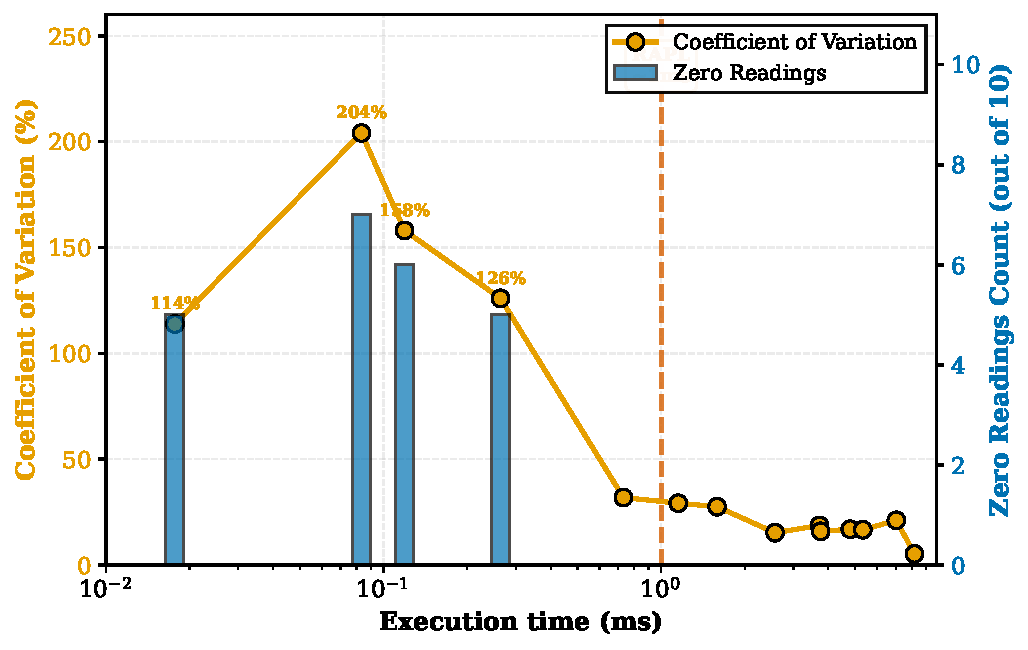
\includegraphics[width=\linewidth]{figures/rapl_paper_quality.pdf} 
  \caption{Quality of RAPL's Measurements over Execution Time of the Workload (ms in Log scale)}
  \label{fig:rapl-quality}
\end{figure}
\section{Motivation}
\label{sec:motivation}
% 1. The Core Challenge in detail 
% A Motivation Example

Developing energy efficient software would require reliable insight into how individual fragments of source code contribute to energy consumption. Existing measurement techniques use hardware based counters such as Intel's Running Average Power Limit (RAPL). While effective for coarse grained profiling, but RAPL's millisecond resolution is too large for such code fragments. As Figure~\ref{fig:rapl-quality} demonstrates that workloads under 1ms register more than 110\% variation and 4-5 runs get zero readings (out of 10 runs). Even above 1ms, the variation is significant. Although hardware power meters provide higher resolution, they are severely limited in terms of accessibility, reproducibility, and usability in distributed systems. To address this fundamental limitation, we developed \textbf{PowerLens}, a methodology for obtaining precise and reproducible energy readings at sub-millisecond granularity. However, accurate measurements alone are insufficient; developers need energy information before code execution. To enable this, we propose \textbf{EnCoDe}, which trains machine learning models on PowerLens measurements to predict block-level energy consumption directly from source code features, shifting energy assessment from a runtime profiling concern to a proactive design-time estimation.

 % \cite{ALVI2021100594} \cite{inproceedings} \cite{10.1145/2425248.2425252}

\begin{comment}

\begin{figure*}[htbp]
  \centering
  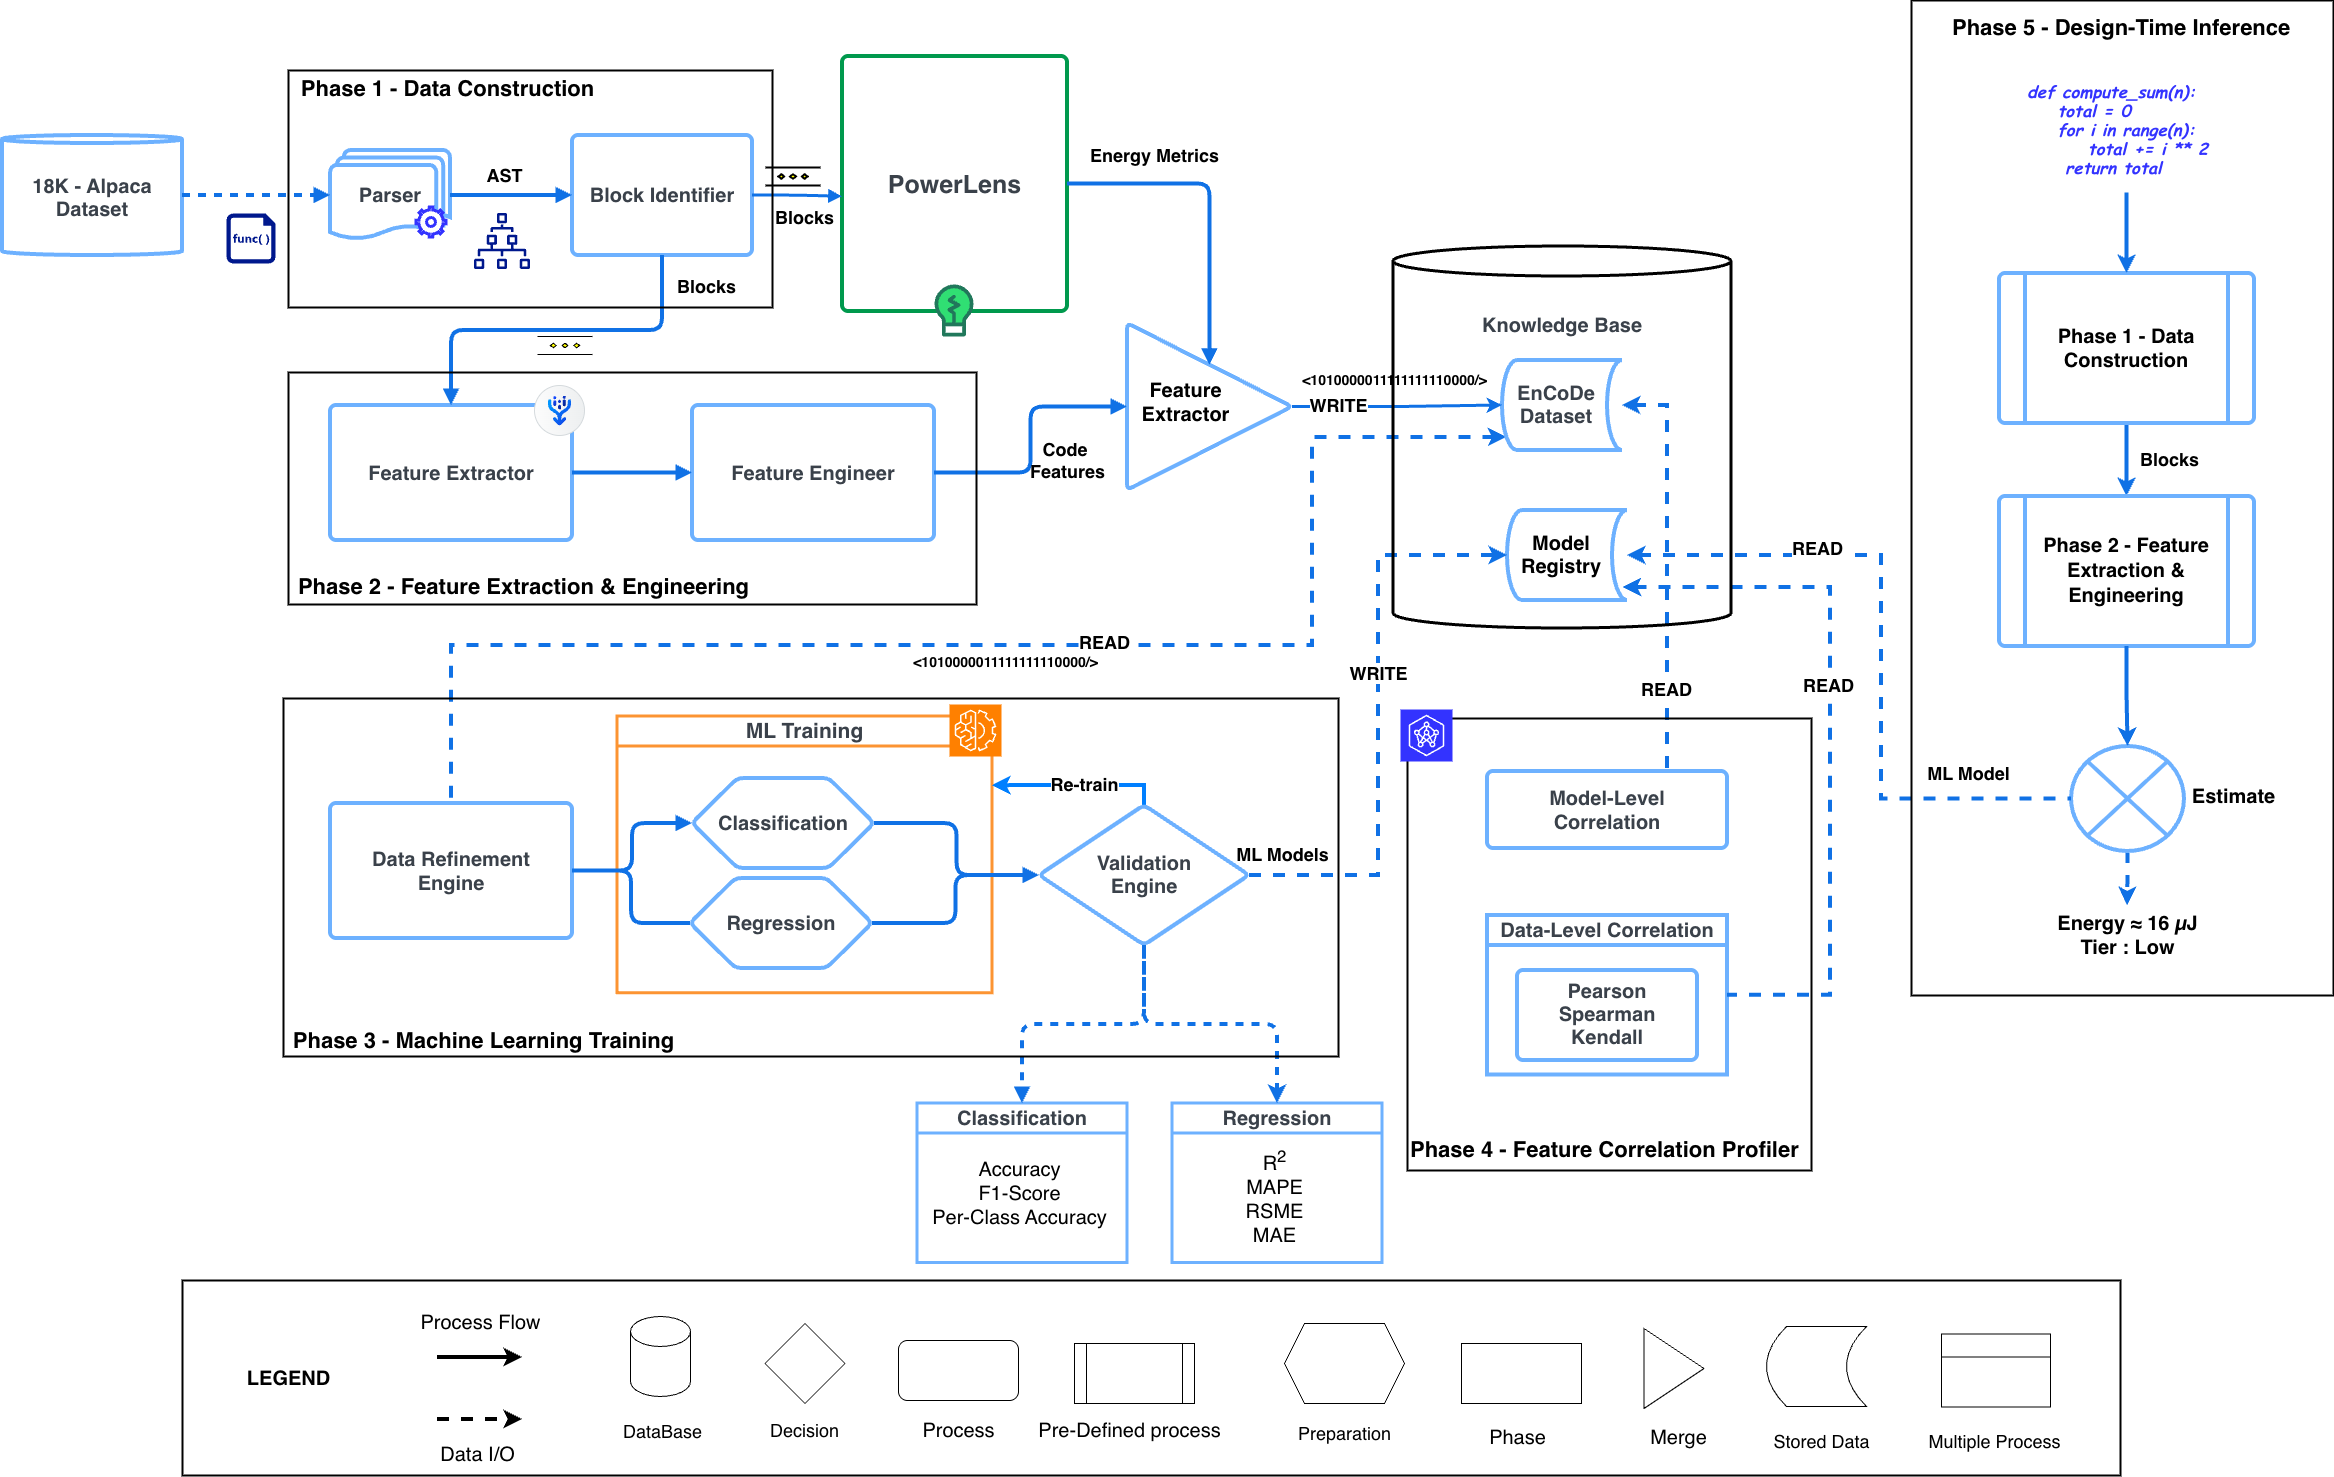
\includegraphics[width=0.95\textwidth]{figures/EnCoDe.png}
  \caption{Design Time Energy Estimation Framework}
  \label{fig:framework}
\end{figure*}

\end{comment}
\section{Methodology}
\label{sec:methodology}

% Architectural Overview. Begin with High-Level Diagram and then briefly walk into the main stages. 
% Implementation and Experimental Setup is seperate section. Introduce the Research Questions here. 

This section details the methodology leveraged by \textit{EnCoDe}. It is organized into a sequence of phases, beginning with the creation of a ground-truth dataset via our novel \textit{PowerLens} measurement methodology, followed by feature extraction, and culminating in the training of predictive models. 

To further explain the methodology followed in detail, we will use the following simple running example of a  Python function (\textit{Listing \ref{lst:calculate_score}}), demonstrating how it is transformed from raw code into a final energy estimate.

\begin{listing}[ht]
\centering
\begin{tcolorbox}[
    colback=codebg,
    colframe=framecol,
    arc=5mm,
    boxrule=1pt,
    title=\textbf{Example: \texttt{score\_function.py}},
    coltitle=black,
    fonttitle=\bfseries,
    top=1mm, bottom=1mm, left=2mm, right=2mm
]
\begin{lstlisting}[language=Python, basicstyle=\small\ttfamily, breaklines=true]
def calculate_score(items, threshold):
    score = 0
    for item in items:
        if item > threshold:
            score += (item * 2)
    return score
\end{lstlisting}
\end{tcolorbox}
\caption{Example: score computation function in Python}
\label{lst:calculate_score}
\end{listing}


\begin{figure*}[htbp]
  \centering
  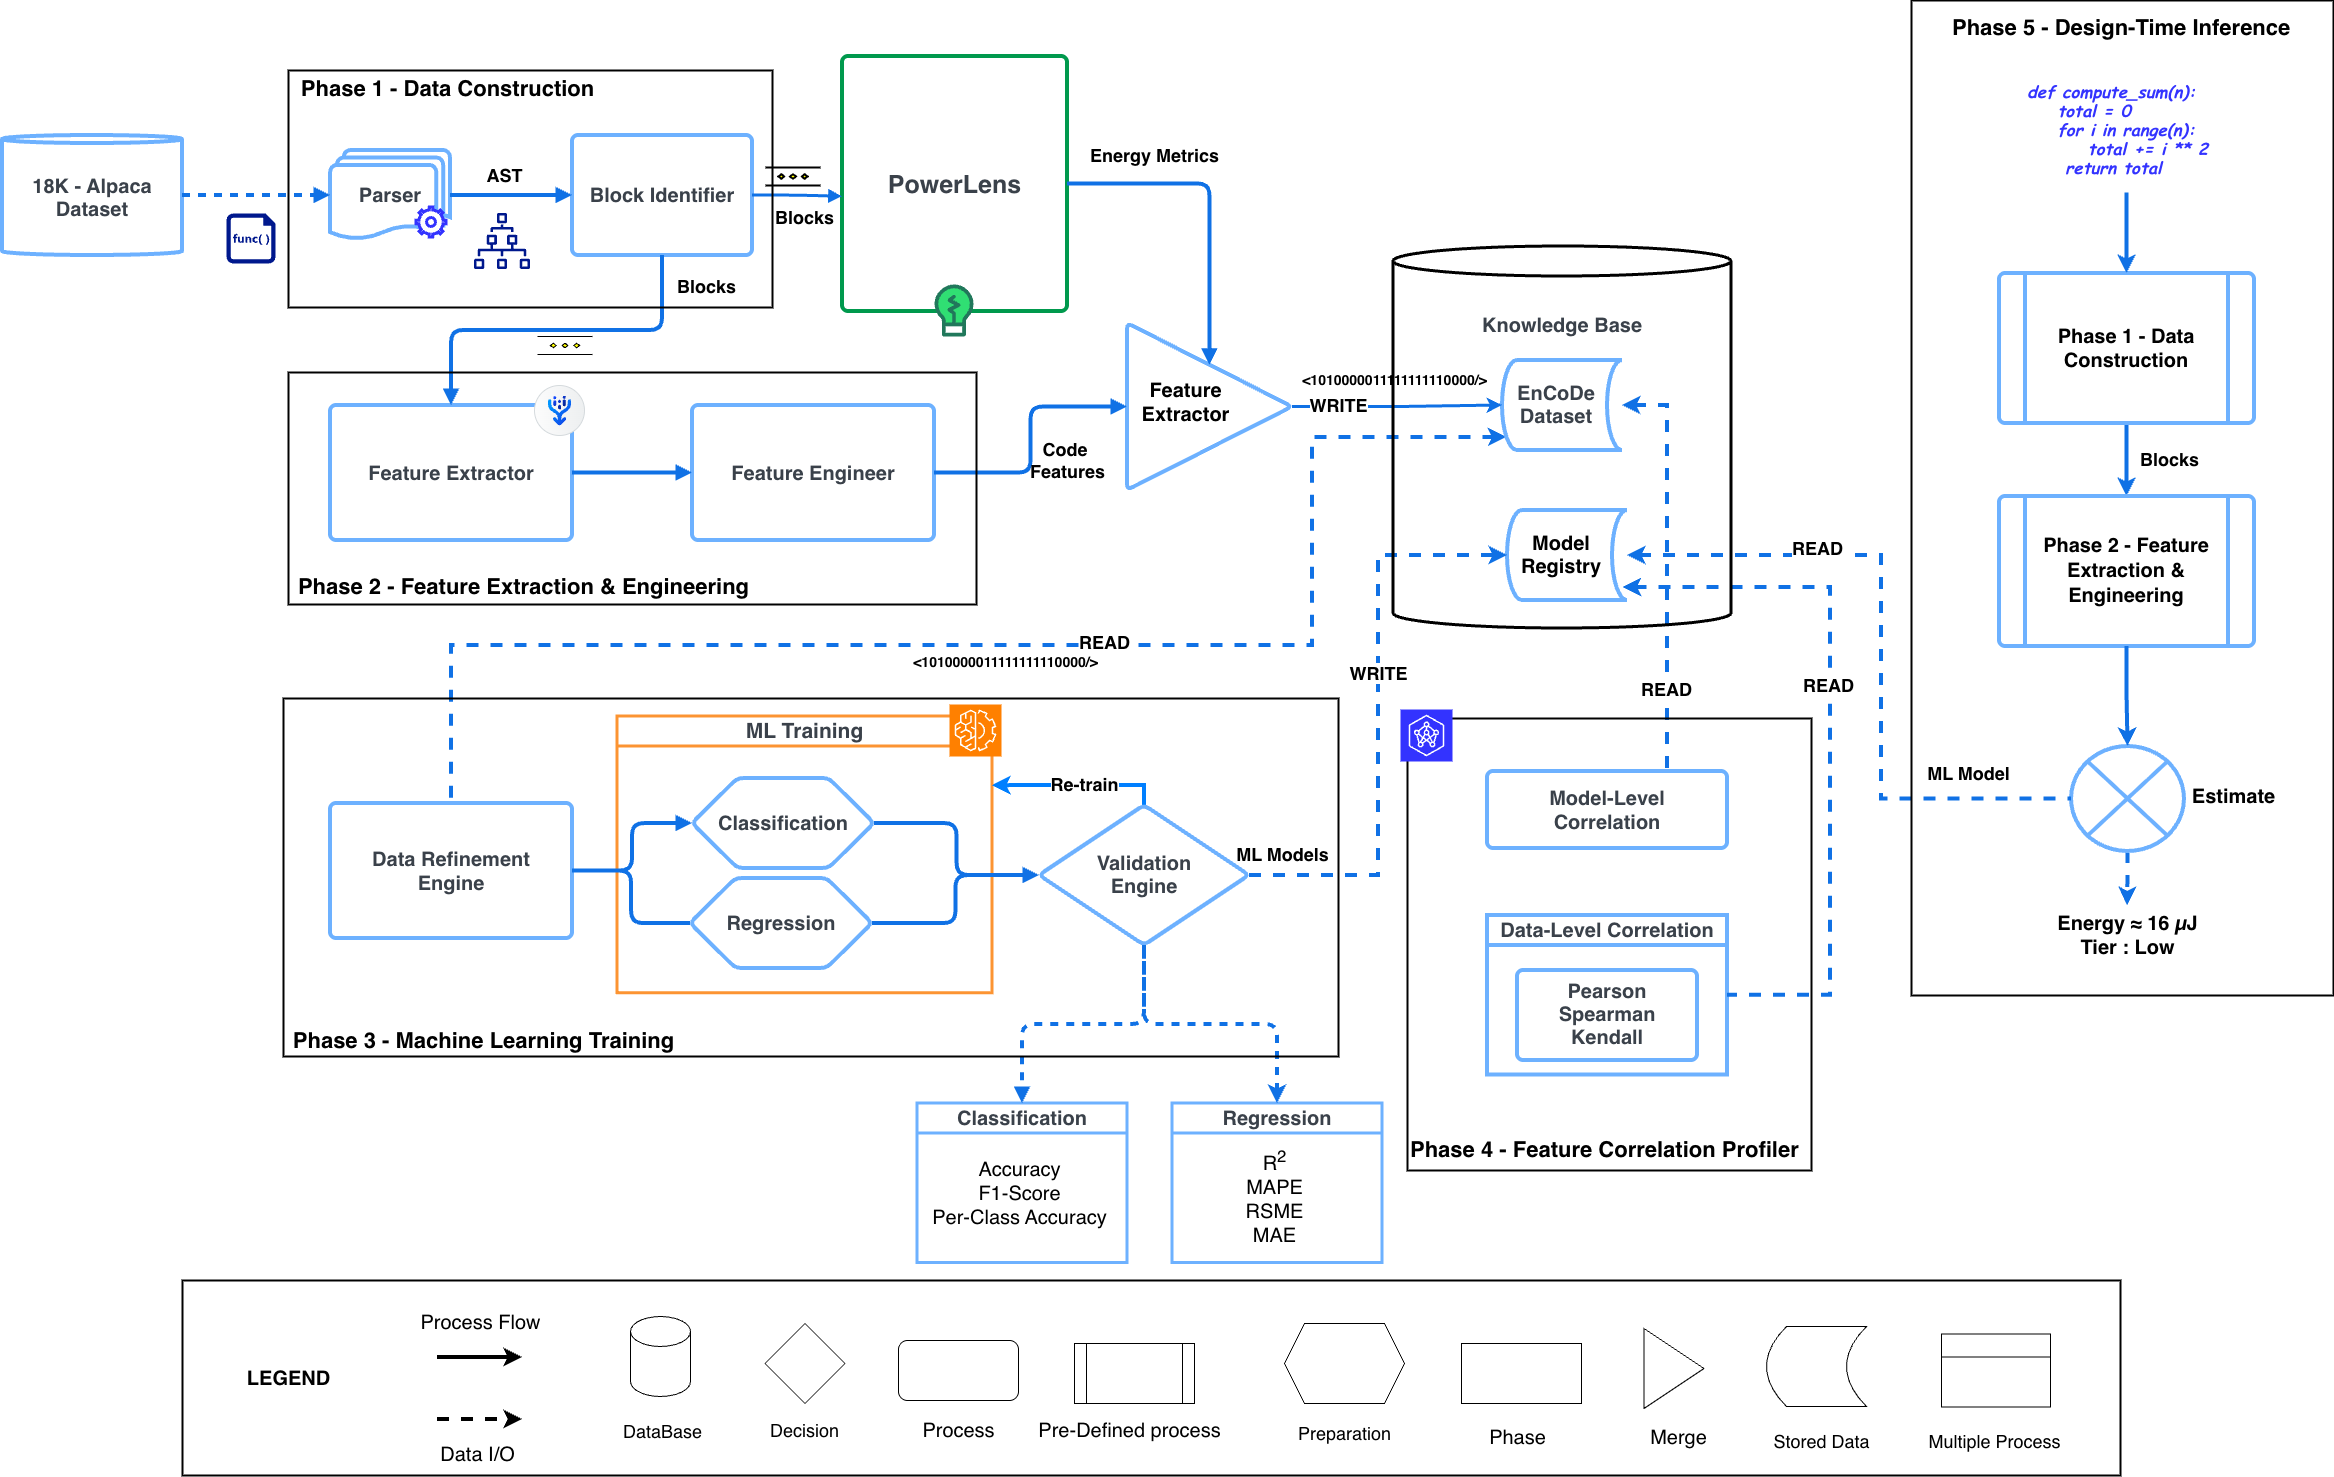
\includegraphics[width=0.95\textwidth]{figures/EnCoDe.png}
  \caption{Design Time Energy Estimation Methodology}
  \label{fig:framework}
\end{figure*}



% This function contains several distinct computational units (blocks) such as a function definition (\textit{def}), a loop (\textit{for}), and a conditional (\textit{if}), whose individual energy contributions are precisely what \textit{EnCoDe} is designed to analyze. 

\subsection{Phase 1 - Data Construction}
\noindent
The first phase of our methodology, as shown in \textit{Figure \ref{fig:framework}}, transforms a raw program text into a structured, analyzable computational block. This is achieved by first parsing the source code \(\mathcal{P}\) to its \textbf{Abstract Syntax Tree (AST)}, a hierarchical representation of the code's structure\cite{Aho1986CompilersPT, sun2023abstractsyntaxtreeprogramming}, as shown in \textit{Figure \ref{fig:block_identification}}. We then traverse the AST to identify node types that represent the root of distinct blocks. We define these block-rooting node types as:

\[ \mathcal{V}_{block} = \{FunctionDef, For, While, If, Try, With\} \]

Each node of these types, along with the entire subtree rooted at that node, is designated as a distinct block, as shown in \textit{Figure \ref{fig:block_identification}}. 

% For example, after parsing our \textit{Listing \ref{lst:calculate_score}} into its AST, this phase identifies all nodes whose types match our defined set of block-rooting nodes (\( \mathcal{V}_{block} \)). This process yields three distinct, nested blocks, each corresponding to a specific AST subtree:

% \begin{itemize}
%     \item \textbf{B0}: Root node of the AST (module level)
%       \begin{itemize}
%         \item \textbf{B1}: \textit{FunctionDef}(\texttt{calculate\_score})
%           \begin{itemize}
%             \item \textbf{B2}: \textit{For} loop inside the function
%               \begin{itemize}
%                 \item \textbf{B3}: \textit{If} statement inside the loop
%               \end{itemize}
%           \end{itemize}
%       \end{itemize}
% \end{itemize}

For \textit{Listing~\ref{lst:calculate_score}}, this yields three nested blocks: B1 (\textit{FunctionDef} \texttt{calculate\_score}), B2 (\textit{For} loop), and B3 (\textit{If} statement inside B2), preserving their containment hierarchy.

The output of this phase is a collection of AST subtrees, each treated as an atomic block. Crucially, their hierarchical context is preserved (e.g., we know B3 is nested within B2), which is essential for all subsequent measurement and feature extraction. 


\begin{figure*}[htbp]
  \centering
  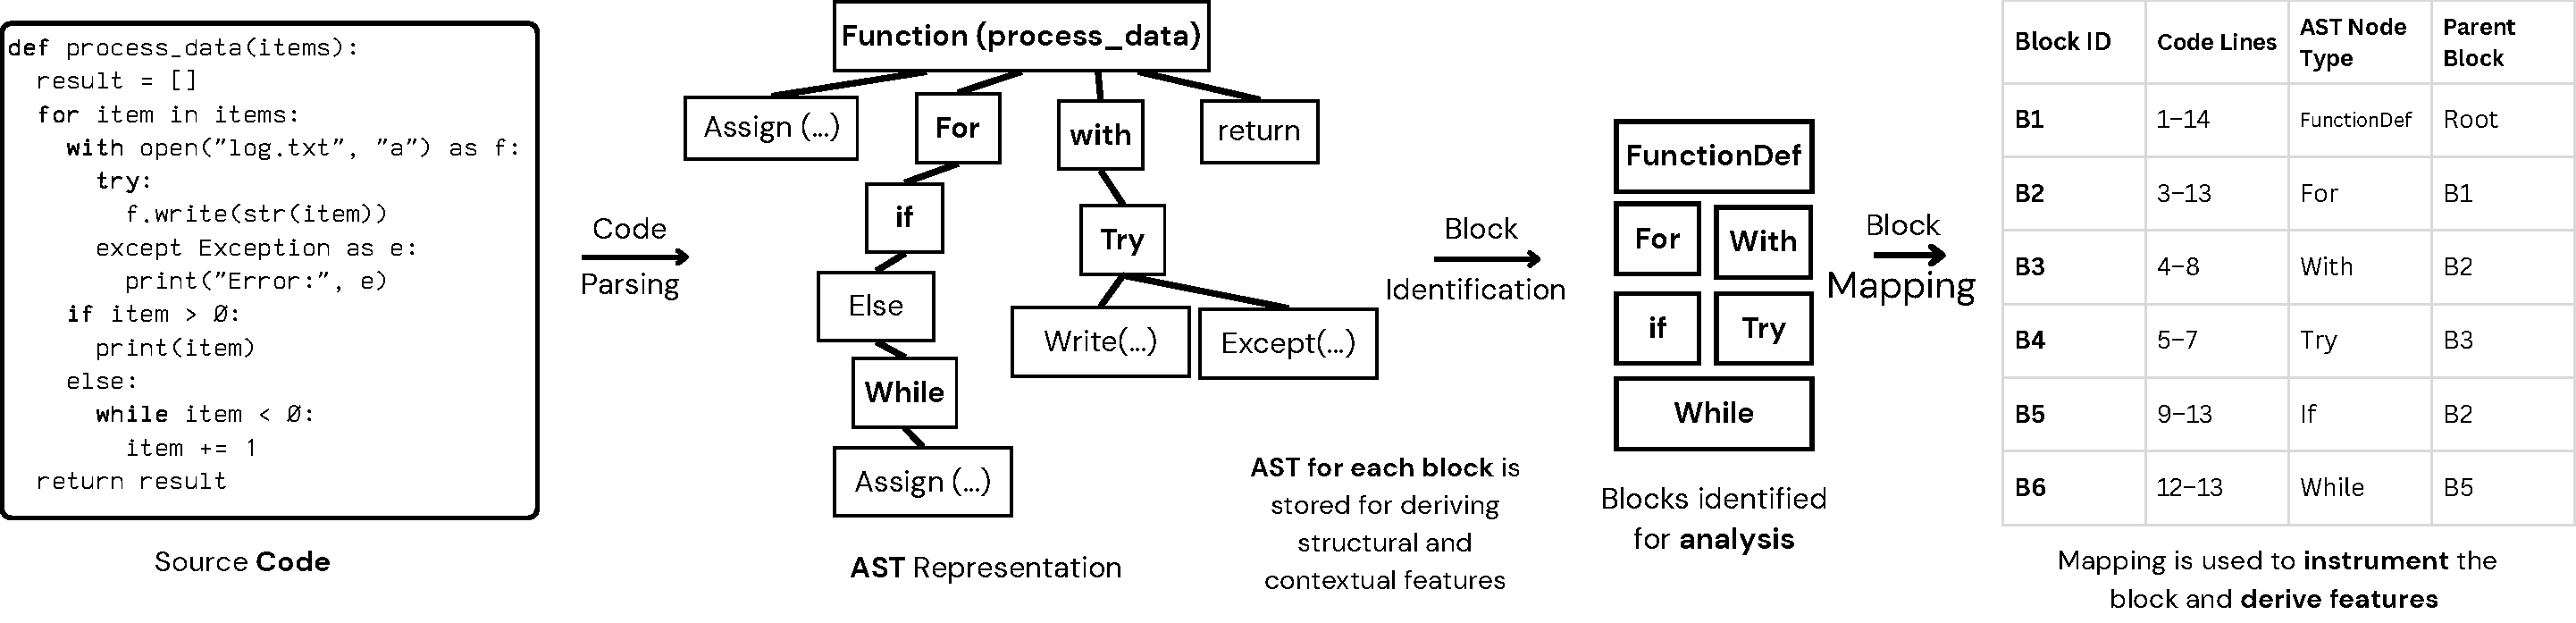
\includegraphics[width=0.95\textwidth]{figures/block_identification.pdf}
  \caption{Code Parsing to identify blocks from AST}
  \label{fig:block_identification}
\end{figure*}
\begin{figure*}[htbp]
  \centering
  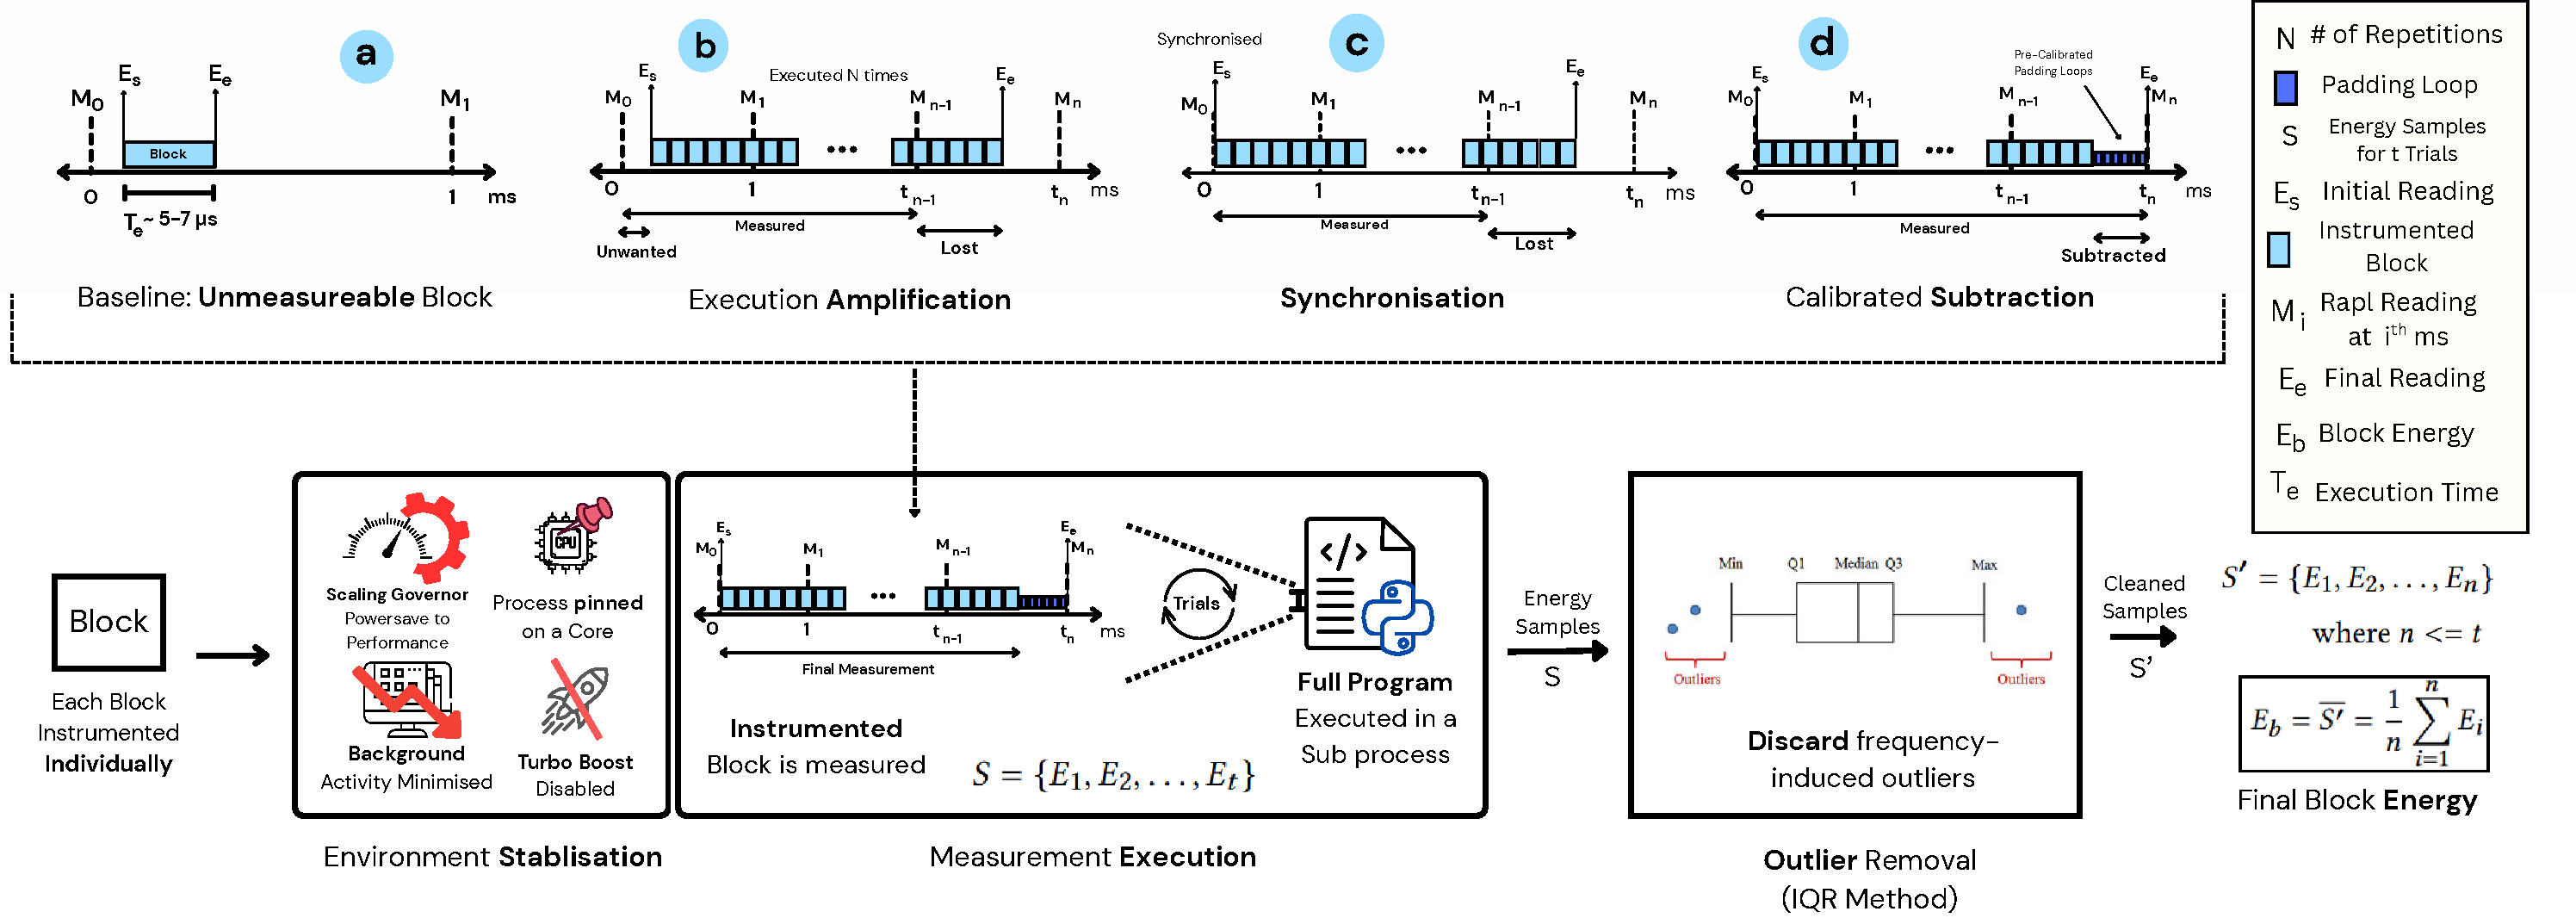
\includegraphics[width=0.95\textwidth]{figures/powerlens.pdf}
  \caption{PowerLens : Sub-Millisecond Energy Measurement Methodology}
  \label{fig:powerlens}
\end{figure*}
% \begin{figure}[t]
%   \centering
%   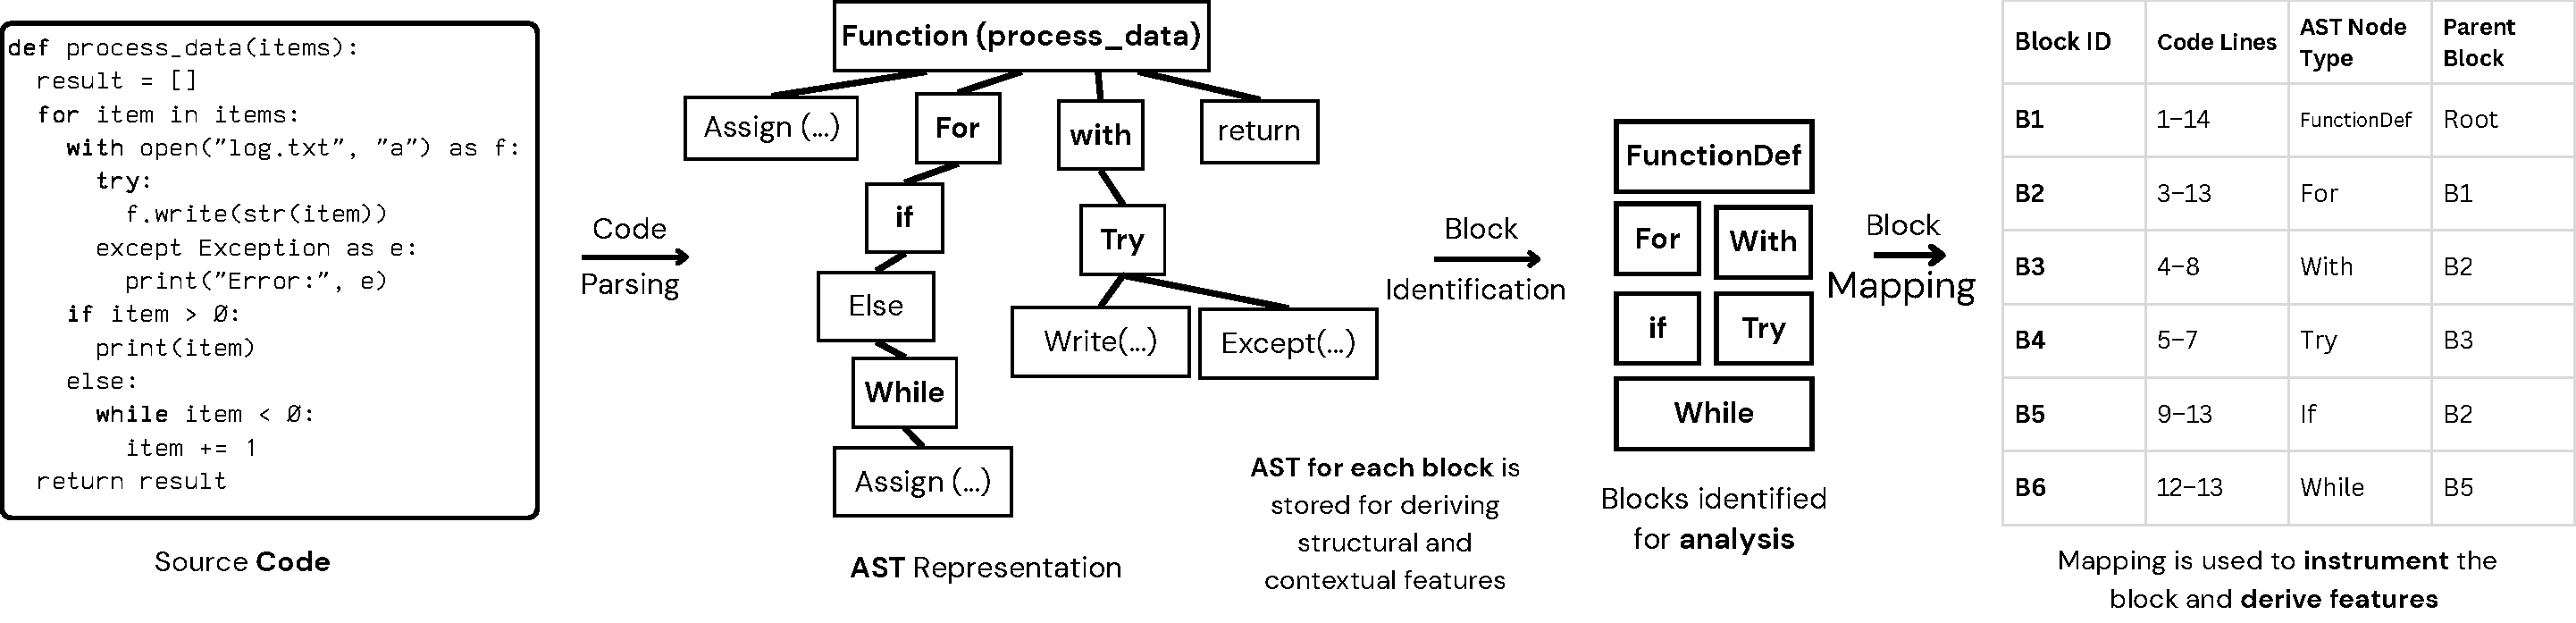
\includegraphics[width=\linewidth]{figures/block_identification.pdf}
%   \caption{Code Parsing to identify blocks from AST}
%   \label{fig:block_identification}
% \end{figure}
% \begin{figure}[t]
%   \centering
%   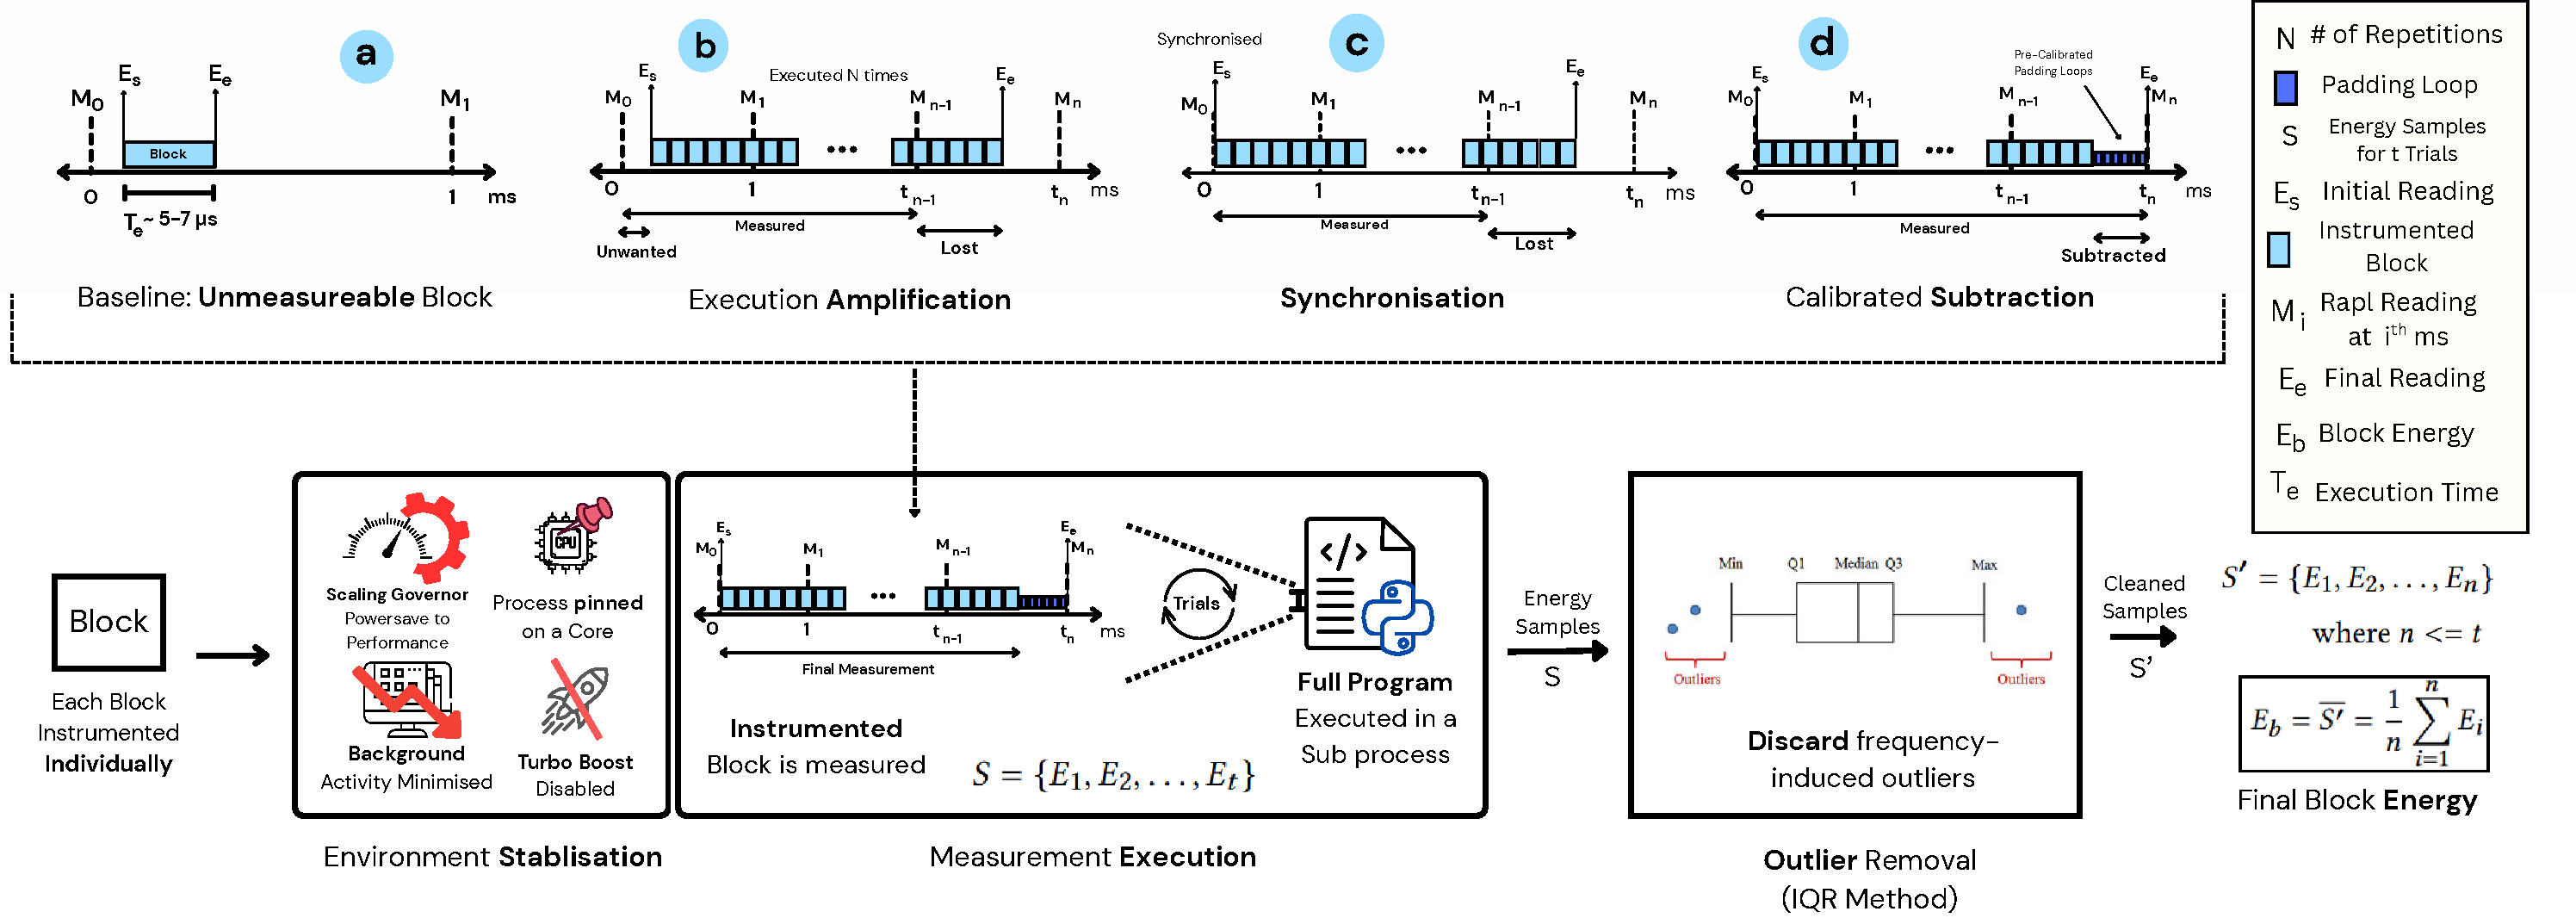
\includegraphics[width=\linewidth]{figures/powerlens.pdf}
%   \caption{PowerLens: Sub-Millisecond Energy Measurement Methodology}
%   \label{fig:powerlens}
% \end{figure}

\subsection{PowerLens: Fine-Grained Energy Measurement}

With the code blocks identified, \textit{PowerLens} measures their energy consumption to create our ground-truth dataset. This is the core technical challenge of our work: a block like the \textit{if} statement (B3) as mentioned in our phase 1, executes in microseconds, far too fast for standard hardware counters like Intel's RAPL to measure directly \cite{ 10.1145/2425248.2425252}. Existing tools, therefore, cannot provide this data, as discussed in related work. \textit{PowerLens} addresses this fundamental measurement 
problem by extending prior work~\cite{10.1145/2425248.2425252}, operating 
through four coordinated mechanisms.

\subsubsection{Environmental Stabilization}
\label{sec:enviromental_Stab}
To ensure measurements are stable, we must isolate the execution from system “noise”. Fluctuations in CPU frequency or background processes can easily distort the tiny energy signature. \textit{PowerLens} enforces a stable environment by setting frequency scaling governor to performance, disabling Turbo Boost, pinning the measurement process to a single core, and suspending non-essential background processes. This ensures that the energy we measure is attributable to the code block itself. 


\subsubsection{Execution Amplification.}

A single execution of a block like our \textit{if} statement (B3) is too fast to register on RAPL's millisecond-scale counters. To make this imperceptible signal measurable, \textit{PowerLens} wraps the target block in a tight loop and executes it \( N \) times. This amplifies the total energy consumed to a level that rises clearly above the millisecond-scale. The total energy \( E_{total} \), is calculated by taking two snapshots of the RAPL energy counter:\( (E_s) \) taken before the execution window, and \( (E_e) \) taken immediately after, as shown in \textit{Figure \ref{fig:powerlens}}. The measured difference is modeled as: 

\[ E_{total}(b, N) = E_e - E_s = N * E(b) + \epsilon_N \]

where \( E_b \) is the true energy of a single execution and \( \epsilon_N \) is the measurement noise which becomes negligible when averaged over N repetitions. By linear aggregation, the estimated mean energy per execution, \( \hat{E(b)} \), becomes:

\[ \hat{E(b)} = \frac{E_{total}(b,N)}{N} \]

For example, to measure B3 as discussed in Phase 1, we execute it N times. If the total measured energy \( E_{total} \) is \( 0.04 \) Joules (J), our initial measurement for a single execution is \( \hat{E}(B3) = 0.04 J / 1000 = 4.0 * 10^{-5} J \). 

\subsubsection{Synchronization - Aligning Execution and Sampling}

Amplification alone is insufficient. If the execution loop starts or end in the middle of a RAPL sampling window, the measurement will be corrupted by energy from unrelated computations, as illustrated by the “unwanted” energy in \textit{Figure \ref{fig:powerlens}}. To solve this, \textit{PowerLens} synchronizes the start of the execution loop with the RAPL counter's refresh cycle.  The start time \( t_0 \) is formally defined as the first moment a counter update is detected after the previous measurement start \( t_s \):

\[ t_0 = min\{ t > t_s | M_{i+1} > M_i \} \]

where \( M_i \) is the cumulative RAPL reading time at time tick \textit{i}. This precise alignment guarantees that the captured energy is attributable only to our target block. 


\subsubsection{Calibrated Subtraction}

As amplified execution rarely finishes exactly on a RAPL boundary, a small “padding” interval is needed to complete the measurement window, and this padding consumes energy that must be removed. \textit{PowerLens} subtracts a pre-calibrated energy cost for this padding, \( E_{pad}(\delta t) \), which is modeled as a linear function of the padding duration \( \delta t \). The final, net energy for a single trial is then:

\[ E_{net}(b) = \frac{E_{total}(b,N) - E_{pad}(\delta t)}{N} \]



\subsubsection{Statistical Aggregation - Achieving Reproducibility}

To ensure the final value is robust against any residual system noise (eg., transient interrupts, SMM), the entire process is repeated \(m (=10)\) times. Outliers are filtered from these trials using the standard \textit{Inter-quartile Range (IQR)} rule \cite{alma9995263502466}. The final energy signature for a block, \( \hat{E(b)} \), is  the mean of the stable, non-outlier observations:

\[ \bar{E}(b) = \frac{1}{|\Omega(b)|} \sum_{i \in \Omega(b)} E_{net}^{(i)}(b) \]

where \(\Omega(b)\) denotes the non-outlier trial set. 

This is applied independently to each block, producing reliable, ground-truth energy values: \(\{B1: 7.7e-2 J, B2: 7.5e-2 J, B3: 1.4e-6 J\}\). This data, which could not be obtained with prior software methods forms our ground truth.

\subsection{Phase 2 - Feature Extraction and Engineering}

After energy measurements, the next step is to create a numerical "fingerprint" for each block based on its source code\cite{10.1145/3639475.3640110}. The goal is to compute a set of static features that capture the block's structural and syntactic characteristics, which we hypothesize are predictive of its energy consumption. This process creates the foundation for our predictive models, as illustrated in \textit{Figure \ref{fig:framework}}.

\subsubsection{Feature Extractor}

This component operates on the AST of each block, computing a feature vector \( x_b \) composed of 33 metrics grouped into seven categories. These categories are designed to capture different facets of code: 

% \smallskip
%\begin{itemize}
\noindent \textbf{Basic Metrics (5)}: Capture the block's overall scale (e.g., AST node count, depth). These serve as a baseline proxy for the total number of components.

% \smallskip
\noindent
\textbf{Complexity Metrics (4)}: Quantify logical intricacy using measures like cyclomatic complexity\cite{1702388}. Prior studies have established a direct correlation between high complexity and increased power consumption, as it often translates to more conditional branches in the instruction stream \cite{Keong2015MetricsPower}.

% \smallskip
\noindent
\textbf{Density Metrics (5)}: Measure the concentration of computational work, such as the ratio of operators to total AST nodes. Dense code regions often correspond to higher instruction throughput and sustained CPU activity.

% \smallskip
\noindent
\textbf{Diversity Metrics (6)}: Assess the heterogeneity of code elements (e.g., entropy of operator types). High diversity may engage a wider range of CPU functional units, influencing micro-architectural energy states.

% \smallskip
\noindent
\textbf{Structural Metrics (3)}: Capture the shape of the control-flow graph (e.g., branching factor), which impacts instruction fetch and branch prediction energy costs. \cite{10.1145/3212695}

% \smallskip
\noindent
\textbf{Code Pattern Metrics (5)}: Identify the presence of semantic constructs like loops and conditionals, which are primary determinants of a block's dynamic execution behavior.

% \smallskip
\noindent
\textbf{Halstead Metrics (5)}: Model the informational complexity of code (e.g., program volume, program effort)\cite{10.5555/540137}. While designed for cognitive effort, Halstead metrics are considered key indicators of software maintainability, a crucial aspect of overall software sustainability and energy efficiency. 

% For example, the \textit{if} statement (B3) is converted into a feature vector. Example
% \emph{ASTDepth} (3),
% \emph{Cyclomatic Complexity} (2),
% \emph{Operator Density} (0.4),
% and a binary flag \emph{HasConditional} (1).


\subsubsection{Feature Integrator}

\noindent
This final component unifies the outputs of the previous phases to produce the EnCoDe Dataset, a key research artifact of this work, as illustrated in \textit{Figure \ref{fig:framework}}. The integrator aligns the feature vector \(x_b\) with the corresponding energy label \(\hat{E}(b)\) for every block.

% \noindent
% For example, the feature vector for the if statement (B3) is paired with its measured energy value Ē(B3) to create a single data point in our dataset: \((x_B3, 1.4e-6 J)\). 



\subsection{Phase 3 - Machine Learning Training}

\noindent
With the finalized EnCoDe dataset, the objective of this phase is to train predictive models that can learn the relationships between a block's static features and its measured energy consumption. We frame this as a supervised learning problem, training two complementary models:
  
\noindent
\textbf{Regression Model \((M_r)\):} This model learns to predict the continuous energy value (in Joules). This allows to precisely compare the expected energy cost of different implementations.

\noindent
\textbf{Classification Model \((M_c)\):} This model provides more intuitive classification into energy tiers. The ground-truth energy values are discretized into three tiers ("Low," "Medium," "High") using equal frequency binning. This provides "lint-like" warning to quickly draw attention to potential energy hotspots. 
% \begin{bluepar}
The classifier's architecture is agnostic to threshold placement,
practitioners can re-bin the training data to match their energy budget
constraints without retraining the feature extraction pipeline.
% \end{bluepar}
\noindent
 To ensure robustness and prevent bias from the skewed energy distribution, models are trained using stratified k-fold cross-validation and checked for overfitting.

\noindent
\textit{For our example:} The data points for our three blocks: \((x_{B1}, 7.7e-2 J)\), \((x_{B2}, 7.5e-2 J)\), and \((x_{B3}, 1.4e-6 J)\), are fed into the training process. The models learn, for instance, that feature vectors with \(HasLoop=1\) and high \(OperatorDensity\) (like \(x_{B2}\)) tend to have higher energy values, while simple conditional blocks (like \(x_{B3}\)) have very low energy.

\subsection{Knowledge Base}
\noindent
The Knowledge Base is the conceptual component in our methodology that stores analytical artifacts, decoupling resource-intensive training from real-time inference.
\noindent
The trained models and the full dataset are stored in the \textbf{Knowledge Base} (Fig.~\ref{fig:framework}), which holds the EnCoDe Dataset \((D_{EnCoDe})\) and a Model Registry containing \(M_r\) and \(M_c\), decoupling resource-intensive training from real-time inference.

\noindent
\textit{For our example:} The data point \((x_B3, 1.4e-6 J)\) for our if statement, along with the data for B1 and B2, is stored in the dataset. The trained models, \(M_r\) and \(M_c\), which have learned from these and thousands of other examples, are stored in the registry.

\subsection{Phase 4 - Feature Correlation Profiler}
\noindent
% A predictive model, even an accurate one, is of limited use if it functions as an unexplainable "black box." To trust our models and to provide developers with actionable insights, we must understand which code characteristics are the most significant drivers of energy consumption. 
The purpose of this phase is to provide crucial interpretability of the prediction models.
\noindent
To achieve this, we perform a dual analysis that cross-validates our findings: one perspective is derived from the trained model's behavior, and the other from direct statistical evidence in the data.
\noindent
\textbf{Model-Based Feature Importance:} First, we analyze the trained models to rank features based on how much they contribute to prediction accuracy. For tree-based ensembles, a feature's influence \(I(f_j)\) can be quantified as its average marginal reduction in prediction error across all decision trees in the model :
\[ I(f_j) = \mathbb{E}_{f \in \mathcal{F}}[\Delta Err(f_j)] \]

\noindent
\textbf{Data-Level Correlation:} Second, we perform a model-agnostic statistical analysis where we compute the correlation coefficients between  features and the measured energy values to capture different types of relationships: Pearson \((\rho_p)\) for linear \cite{1896RSPTA.187..253P}, Spearman \((\rho_s)\) for monotonic \cite{spearman04}, and Kendall \((\rho_k)\) for rank-based associations\cite{665905b2-6123-3642-832e-05dbc1f48979}. This collection of correlations is represented as:
\[ \mathcal{C} = \{ (f_j, \rho_p(f_j, E)), (f_j, \rho_s(f_j, E)), (f_j, \rho_k(f_j, E)) \} \]

\noindent
By confirming that both analyses highlight the same key features, we increase our confidence that the models are capturing genuine, underlying relationships between code structure and energy, rather than learning from spurious artifacts.

\noindent
\textit{For our example:} This dual analysis provides deep insights.


\noindent
For the \textit{for} loop (B2), the feature importance might rank the binary feature \(HasLoop=1\) and the \(CyclomaticComplexity\) metric very highly.
\noindent
Simultaneously, the data-level analysis would likely show a strong positive Spearman correlation \((\rho_s)\) between these same features and energy across the entire dataset.
\noindent
This convergence gives us high confidence that the model has correctly learned a fundamental truth: loops and complex logic are significant drivers of energy consumption. The profiler's output is a unified ranking of these influential features, bridging the gap between prediction and explanation.

\subsection{Phase 5 - Design-Time Inference}
\noindent
This phase operationalizes EnCoDe's goal of design-time energy estimation by translating static code blocks into predictions using pre-trained models.
\noindent
The inference engine takes a newly written or modified code block as input and performs the following steps, as in \textit{Figure \ref{fig:framework}} :

    
\noindent
\textbf{Block Identification and Feature Extraction:} The unseen code is parsed into its AST, and its constituent blocks are identified using the same mechanism as in Phase 1. The Feature Extractor from Phase 2 is then reused to compute the corresponding feature vector, \(x_b^{new}\), for each new block.

\noindent
\textbf{Model-Based Prediction:} The pre-trained regression (\(M_r)\) and classification \((M_c)\) models are retrieved from the Model Registry in the Knowledge Base by the inference engine to generate the predictions.

\noindent
Formally, the inference process can be represented as a transformation function \(\Phi\) that maps the new block \(b_{new}\) and the stored models to an energy estimate and a tier : 
% \[Φ: (b_{new}, M_r, M_c) → (\hat{E}_b, T_b)\]
\begin{equation}
\Phi \colon (b_{\text{new}}, M_r, M_c) \to (\hat{E}_b, T_b)
\end{equation}


\noindent
where \(\hat{E}_b\) is the predicted energy in Joules and \(T_b\) is the predicted tier (e.g., "Low," "Medium," "High"). Crucially, this entire process is static and does not require any code execution. 

\noindent
\textit{For our example:} Imagine a developer is refactoring our Listing \ref{lst:calculate_score} function and replaces the for loop (B2) with a while loop.
 As they finish writing the new while loop block, energy is inferred again. The regression model \(M_r\) might predict an energy value of \(\hat{E}_b = 6.9e-2 J\). Simultaneously, the classification model \(M_c\) might predict the tier \(T_b\) = "Medium".
% \noindent
% This feedback, either the precise numerical estimate or the intuitive "Medium" tier warning, can then be displayed directly in the developer's editor, fulfilling the goal of design-time energy awareness.





\section{Experimental Setup}
\label{sec:exp-setup}
All experiments were executed on a dedicated, isolated machine under controlled conditions to maximize measurement stability and reproducibility.

\textbf{Hardware and system environment.}
Experiments were performed on an Intel CPU (model: \texttt{i7-6700K}; with 16\,GB DDR4 RAM, running Pop!\_OS 22.04 (64 bit). To reduce measurement noise, we stabilized the environment as in Section \ref{sec:enviromental_Stab}. We loaded the \texttt{msr} kernel module to access Model-Specific Registers for RAPL readings.


\textbf{Software environment.}
All experiments used Python~3.12. Block extraction relied on the standard \texttt{ast} module and custom instrumentation utilities. All code, experiment scripts, and seed values for pseudo-random operations are archived and available in the artifact repository. We set a fixed random seed for all learning experiments to ensure reproducible train/test splits and model initializations.

\textbf{Dataset.}
The dataset was constructed from a larger corpus of Python programs\footnote{\url{https://huggingface.co/datasets/iamtarun/python_code_instructions_18k_alpaca}}. After parsing with \texttt{ast}, we extracted executable code blocks defined as function bodies, loop bodies (\texttt{for}, \texttt{while}), conditional bodies (\texttt{if}), exception handlers (\texttt{try/except}), and context manager blocks (\texttt{with}). We filtered out non-executable blocks as we need ground truth measurements. From \textbf{18,612} code files, we extract \textbf{14,000+} executable blocks, retaining \textbf{8,000+} that exceed 1 µs (measurable with N=1000). Each block was annotated with a set of \textbf{33 static features} comprising of AST derived features and standard code properties.

\textbf{Measurement protocol.}
Energy readings were taken from processor energy counters exposed via Intel RAPL through MSR access. Specifically, we read the \texttt{PACKAGE} domains using the MSR interface. All MSR reads were executed with root privileges and synchronized with our measurement control loop to avoid partial-window reads. 
Block execution times are typically in the microsecond range, while RAPL updates at millisecond granularity; to bridge this mismatch we used deterministic amplification and synchronization as follows:

% \begin{enumerate}

%   \item \textbf{Amplification:} each target block was executed in a tight loop of $N$ consecutive iterations (we used $N=1000$), and the total energy measured across the loop was divided by $N$ to yield a per-iteration estimate. The value of $N$ was chosen to produce a signal that is reliably captured by RAPL while keeping total runtime reasonable.
%   \item \textbf{Synchronization and padding:} before starting an amplification loop we ensured the RAPL counters had updated (fresh window) and, after the loop, appended a calibrated empty loop (padding) whose energy cost was measured separately and subtracted from the aggregate reading to compensate for loop/overhead energy.
%   \item \textbf{Repetitions and outlier-handling:} Each amplified measurement was repeated $m=10$ times; we discarded statistical outliers using interquartile-range (IQR) filtering and used the mean of the remaining trials as the final block energy estimate. The outliers occured due to randomly occuring system flareups that affect energy usage.
%   \item \textbf{Environment stabilization:} between block measurements we allowed a short cool-down period and ensured background system activity remained minimal. The CPU governor remained set to \texttt{performance} throughout; Turbo Boost and other dynamic frequency controls were disabled to avoid transient frequency-induced variability.
% \end{enumerate}

% \paragraph{Baseline validation.}
% To validate aggregated block-level energy, we compared summed PowerLens measurements against coarse-grained program-level energy reported by PyRAPL (or an equivalent RAPL wrapper). The aggregated block sums were consistent with PyRAPL measurements across block categories (see Figure~\ref{fig:powerlens-pyrapl}).

\textbf{Evaluation protocol and statistical analysis.}
We evaluated both regression and classification formulations. Regression performance metrics include R² (variance explained), RMSE (root mean squared error), MAE (mean absolute error), and MAPE (mean absolute percentage error) \cite{Botchkarev2018PerformanceM}\cite{Chicco2021TheCO}. For classification (energy-tier prediction), we report accuracy (correct predictions), precision (positive prediction accuracy), recall (true positive coverage), F1-score (harmonic mean of precision and recall), and confusion matrices \cite{SOKOLOVA2009427}. All reported results include mean and standard deviation across folds.


% \begin{figure}[t]
%   \centering
%   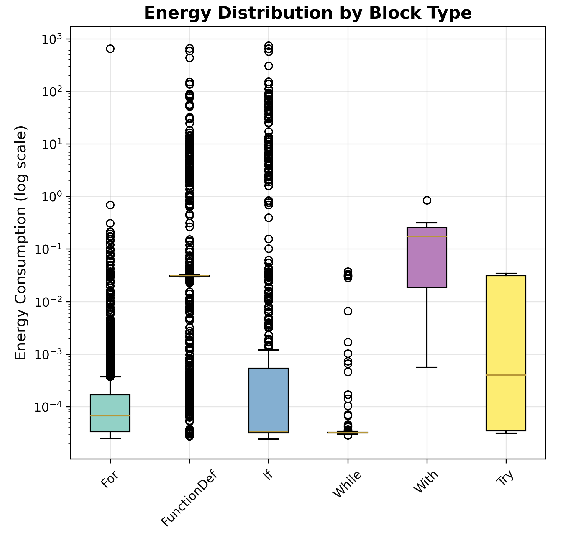
\includegraphics[width=0.9\linewidth]{figures/energy_distribution_by_block_type.png}
%   \caption{Energy consumption distribution across different block types.}
%   \label{fig:energy-distribution-block-type}
% \end{figure}

\section{Research Questions}
\label{sec:research-questions}

% Our work addresses the overarching problem of how energy efficiency can be made a design time concern for software developers.
To guide our investigation, we formulate the following three research questions. These questions are answered through the analyses presented in Section~\ref{sec:results}.

\textbf{RQ1: How can energy consumption of small code blocks be measured accurately and reproducibly?}  
We evaluate the proposed methodology's measurement granularity, stability and effectiveness for small code blocks.

\textbf{RQ2: What statistical relationships exist between static code features and block-level energy consumption?}  
We investigate whether code structure and metrics are statistically related to energy consumption. This leads to two sub-questions:
\begin{itemize}
  \item \textbf{RQ2a}: Which static code features exhibit associations with block's energy consumption?  
  \item \textbf{RQ2b}: What is the nature of these associations between energy consumption and code features?
  %   \item \textbf{RQ2a}: What kind of code aspects have high impact on block's energy consumption?  
  % \item \textbf{RQ2b}: How do structural and contextual features derived from Abstract Syntax Trees correlate to energy?
\end{itemize}
% These are answered through correlation analyses (Pearson, Spearman, Kendall) and feature importance rankings across features.

\textbf{RQ3: How reliably can code features predict block-level energy consumption?}  
Beyond correlation, we ask whether predictive models trained on static features can predict energy consumption and generalize to unseen code. This leads to two sub-questions:
\begin{itemize}
  \item \textbf{RQ3a:} How accurately can regression models predict absolute block-level energy values?  
  \item \textbf{RQ3b:} How effectively can classification models assign blocks to energy tiers (low, medium, high)?  
\end{itemize}
% These are answered through regression and classification performance metrics, cross-validation stability, and analysis of generalization gaps between training and test sets.

% These questions are answered through the implementation of our Visual Studio Code extension, which highlights energy-intensive blocks inline with source code, enabling targeted refactoring at design time.


\section{Results}
\label{sec:results}


We present the results according to the research questions defined in Section ~\ref{sec:research-questions}.

\subsection{RQ1: How can energy consumption of small code blocks be measured accurately and reproducibly?}

\begin{figure}[t]
  \centering
  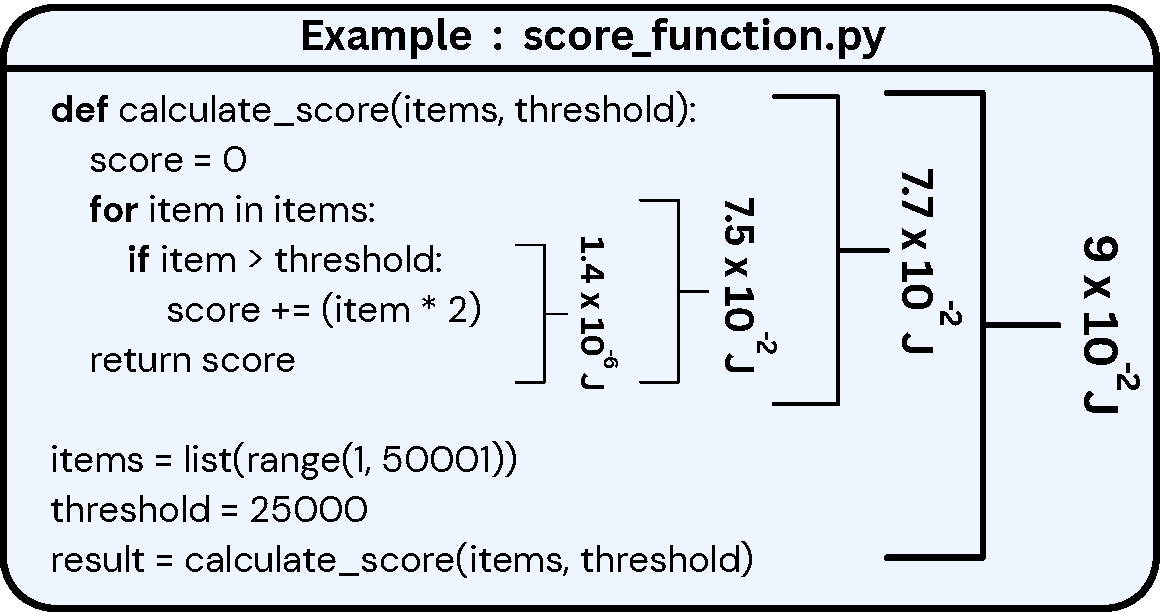
\includegraphics[width=1\linewidth]{figures/example_measurement.pdf}
  \caption{Block Level Energy Measurement of the score computation function}
  \label{fig:example-measurement}
\end{figure}
Our first research question examines whether energy consumption of microsecond-scale code blocks can be measured accurately and reproducibly.  Each block was measured ten times, and across the dataset \textbf{more than 90\%} of the blocks exhibited \textbf{less than 10\% variation} between repeated trials after IQR outlier removal, indicating strong measurement stability and effective suppression of environmental noise. The results demonstrate that the proposed measurement infrastructure provides stable and reliable energy values at block granularity. This is a result of system stabilization and calibrated padding loops.

The measurement protocol also achieves both high sensitivity and broad coverage. The observed energy values spans six orders of magnitude, ranging from $2.37 \times 10^{-5}$ joules for trivial blocks to $7.48 \times 10^{2}$ joules for complex functions. This wide dynamic range confirms that the methodology is capable of capturing energy signatures of extremely short-lived constructs while remaining reliable. Without the amplification and synchronization mechanisms, many of these fine-grained blocks would register highly unstable or zero readings using conventional software-profilers.

Figure~\ref{fig:example-measurement} illustrates block-level energy measurements for the \texttt{score\_function.py} example, where annotated values indicate per-block energy consumption in joules as measured by PowerLens in Nested Blocks.
Figure~\ref{fig:powerlens-pyrapl} compares the sum of block-level energy measurements obtained with PowerLens against coarse-grained measurements from PyRAPL\footnote{\url{https://github.com/powerapi-ng/pyRAPL}}, grouped by construct type. To \textbf{validate} the correctness of the fine-grained measurements, we compared the aggregate energy obtained by summing block-level measurements from PowerLens with the total program-level energy reported by PyRAPL for the same codes, across 40 instances of each block type (see Figure~\ref{fig:powerlens-pyrapl}). For all block categories, the aggregated PowerLens measurements closely match the corresponding coarse-grained energy reported by PyRAPL. In addition, PowerLens exhibits \textbf{substantially lower variance} across repeated measurements, as it stabilizes the execution environment and applies calibration loops to isolate block execution energy.
% These results confirm that \textbf{PowerLens} provides \textbf{reliable, high-resolution} energy measurements across diverse code constructs while remaining consistent with established coarse-grained profiling tools.


\begin{rqbox}{Answer to RQ1}Together, these results confirm that PowerLens enables accurate, stable, and reproducible energy measurement at the level of individual small code blocks, overcoming the temporal limitations of existing software-based profilers.
\end{rqbox}

\begin{figure}[t]
  \centering
  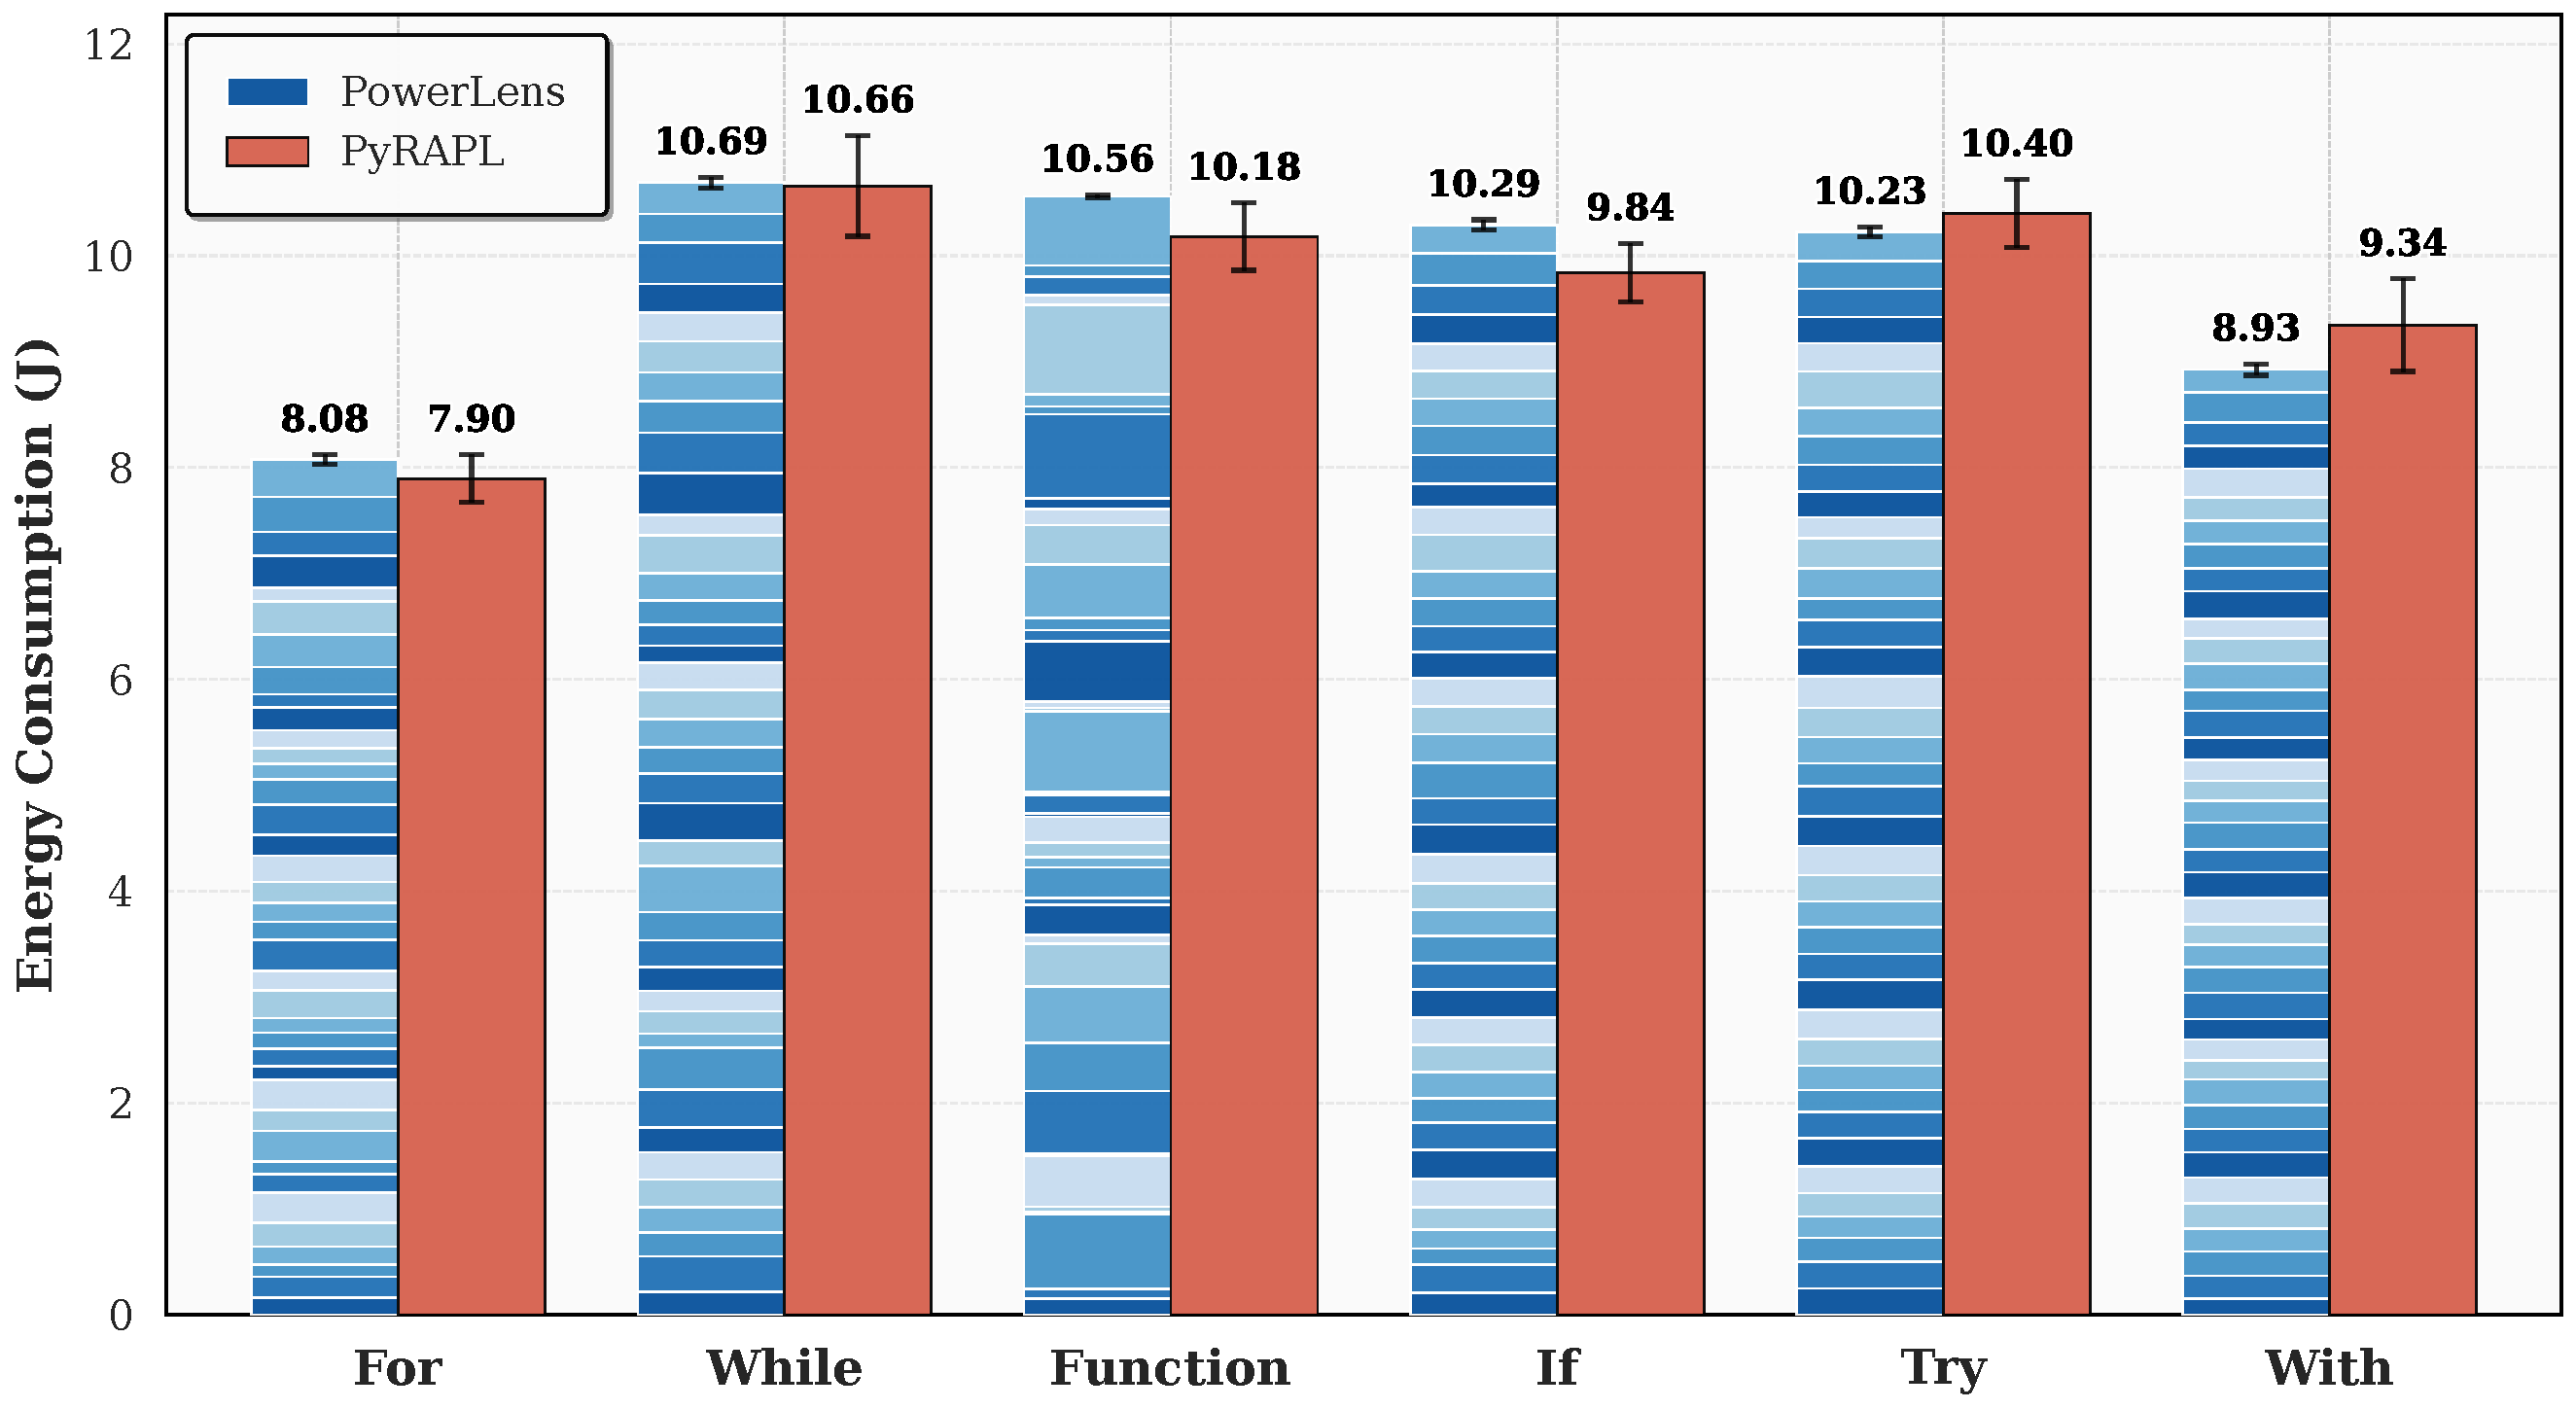
\includegraphics[width=1\linewidth]{figures/validation_plot_hq.pdf}
  \caption{Sum of Blocks measured by Powerlens compared with Overall measurement by Pyrapl}
  \label{fig:powerlens-pyrapl}
\end{figure}
% \textbf{\textit{PLACEHOLDER: Boxplot of measurement variance across blocks; histogram of block-level energy distribution.}}

\subsection{RQ2: What statistical relationships exist between static code features and block-level energy consumption?}


% \begin{table*}[htbp]
% \centering
% \caption{Top 20 features ranked by correlation and model-based importance methods.}
% \resizebox{\textwidth}{!}{%
% \begin{tabular}{c l c l c l c l c l c l c}
% \hline
% Rank & \multicolumn{2}{c}{Pearson ($r$)} & \multicolumn{2}{c}{Spearman ($\rho$)} & 
% \multicolumn{2}{c}{Kendall ($\tau$)} & \multicolumn{2}{c}{Gradient Boost} & \multicolumn{2}{c}{XGBoost} & \multicolumn{2}{c}{Random Forest}\\
% \cline{2-13}
% & Feature & Value & Feature & Value & Feature & Value & Feature & Value & Feature & Value & Feature & Value\\
% \hline
% 1    & \cellcolor[HTML]{A0C3D5}functions count      & 0.704  & \cellcolor[HTML]{A0C3D5}functions count      & 0.616 & \cellcolor[HTML]{A0C3D5}functions count      & 0.503 & \cellcolor[HTML]{A0C3D5}functions count       & 0.620 & \cellcolor[HTML]{A0C3D5}functions count       & 0.410 & \cellcolor[HTML]{A0C3D5}functions count         & 0.273 \\
% 2    & \cellcolor[HTML]{A0C3D5}node type entropy    & 0.434  & \cellcolor[HTML]{A0C3D5}node type entropy    & 0.393 & \cellcolor[HTML]{A0C3D5}node type entropy    & 0.263 & \cellcolor[HTML]{F8CBAD}depth variance        & 0.140 & \cellcolor[HTML]{D4E7C5 }leaves to nodes ratio & 0.062 & \cellcolor[HTML]{A0C3D5}node type entropy       & 0.097 \\
% 3    & \cellcolor[HTML]{A0C3D5}unique node types    & 0.372  & \cellcolor[HTML]{A0C3D5}unique node types    & 0.347 & \cellcolor[HTML]{A0C3D5}unique node types    & 0.243 & \cellcolor[HTML]{D4E7C5 }leaves to nodes ratio & 0.096 & \cellcolor[HTML]{D4E7C5 }call density          & 0.061 & \cellcolor[HTML]{A0C3D5}unique node types       & 0.064 \\
% 4    & \cellcolor[HTML]{F8CBAD}depth variance       & 0.222  & \cellcolor[HTML]{F8CBAD}depth variance       & 0.326 & \cellcolor[HTML]{F8CBAD}max branching factor & 0.243 & \cellcolor[HTML]{D4E7C5 }call density          & 0.087 & \cellcolor[HTML]{A0C3D5}node type entropy     & 0.057 & \cellcolor[HTML]{D4E7C5 }leaves to nodes ratio   & 0.035 \\
% 5    & \cellcolor[HTML]{F8CBAD}max branching factor & 0.218  & \cellcolor[HTML]{F8CBAD}max branching factor & 0.317 & \cellcolor[HTML]{F8CBAD}depth variance       & 0.220 & \cellcolor[HTML]{F8CBAD}variable density      & 0.075 & \cellcolor[HTML]{F8CBAD}depth variance        & 0.049 & \cellcolor[HTML]{F8CBAD}depth variance          & 0.035 \\
% 6    & max depth                                    & 0.192  & max depth                                    & 0.281 & max depth                                    & 0.206 & \cellcolor[HTML]{D4E7C5 }avg depth             & 0.067 & \cellcolor[HTML]{F8CBAD}variable density      & 0.040 & \cellcolor[HTML]{D4E7C5 }cyclomatic complexity   & 0.034 \\
% 7    & \cellcolor[HTML]{D4E7C5 }avg depth            & 0.137  & \cellcolor[HTML]{D4E7C5 }avg depth            & 0.221 & \cellcolor[HTML]{D4E7C5 }avg depth            & 0.148 & \cellcolor[HTML]{A0C3D5}node type entropy     & 0.067 & \cellcolor[HTML]{A0C3D5}unique node types     & 0.037 & \cellcolor[HTML]{D4E7C5 }call density            & 0.033 \\
% 8    & \cellcolor[HTML]{D4E7C5 }total nodes          & 0.114  & \cellcolor[HTML]{D4E7C5 }total nodes          & 0.181 & unique functions                             & 0.126 & \cellcolor[HTML]{D4E7C5 }operator density      & 0.050 & \cellcolor[HTML]{D4E7C5 }avg depth             & 0.035 & \cellcolor[HTML]{D4E7C5 }control flow complexity & 0.032 \\
% 9    & program volume                               & 0.075  & \cellcolor[HTML]{D4E7C5 }avg branching factor & 0.181 & \cellcolor[HTML]{D4E7C5 }total nodes          & 0.125 & \cellcolor[HTML]{D4E7C5 }attribute density     & 0.047 & \cellcolor[HTML]{F8CBAD}max branching factor  & 0.034 & \cellcolor[HTML]{D4E7C5 }cognitive complexity    & 0.032 \\
% 10   & \cellcolor[HTML]{D4E7C5 }avg branching factor & 0.073  & unique functions                             & 0.156 & \cellcolor[HTML]{D4E7C5 }avg branching factor & 0.125 & \cellcolor[HTML]{D4E7C5 }literal density       & 0.031 & \cellcolor[HTML]{D4E7C5 }cognitive complexity  & 0.022 & \cellcolor[HTML]{F8CBAD}max branching factor    & 0.031 \\
% 11   & program length                               & 0.073  & vocabulary size                              & 0.142 & vocabulary size                              & 0.104 & \cellcolor[HTML]{A0C3D5}unique node types     & 0.026 & \cellcolor[HTML]{D4E7C5 }operator density      & 0.022 & \cellcolor[HTML]{F8CBAD}variable density        & 0.030 \\
% 12   & unique operators                             & 0.070  & program volume                               & 0.136 & program volume                               & 0.095 & \cellcolor[HTML]{F8CBAD}max branching factor  & 0.022 & \cellcolor[HTML]{D4E7C5 }cyclomatic complexity & 0.018 & \cellcolor[HTML]{D4E7C5 }operator density        & 0.029 \\
% 13   & operator entropy                             & 0.067  & program length                               & 0.128 & loops count                                  & 0.092 & variable entropy                              & 0.018 & \cellcolor[HTML]{D4E7C5 }literal density       & 0.017 & \cellcolor[HTML]{D4E7C5 }nesting complexity      & 0.025 \\
% 14   & program difficulty                           & 0.061  & unique variables                             & 0.114 & program length                               & 0.091 & \cellcolor[HTML]{D4E7C5 }nesting complexity    & 0.017 & \cellcolor[HTML]{D4E7C5 }attribute density     & 0.016 & \cellcolor[HTML]{D4E7C5 }avg depth               & 0.025 \\
% 15   & vocabulary size                              & 0.052  & variable entropy                             & 0.112 & unique variables                             & 0.090 & program difficulty                            & 0.016 & variable entropy                              & 0.014 & \cellcolor[HTML]{D4E7C5 }literal density         & 0.021 \\
% 16   & program effort                               & 0.051  & loops count                                  & 0.110 & variable entropy                             & 0.083 & \cellcolor[HTML]{D4E7C5 }total nodes           & 0.015 & \cellcolor[HTML]{D4E7C5 }total nodes           & 0.014 & \cellcolor[HTML]{D4E7C5 }total nodes             & 0.020 \\
% 17   & \cellcolor[HTML]{D4E7C5 }operator density     & 0.018  & program effort                               & 0.068 & program effort                               & 0.048 & conditionals count                            & 0.012 & \cellcolor[HTML]{D4E7C5 }nesting complexity    & 0.013 & \cellcolor[HTML]{D4E7C5 }avg branching factor    & 0.020 \\
% 18   & \cellcolor[HTML]{D4E7C5 }attribute density    & 0.012  & \cellcolor[HTML]{D4E7C5 }literal density      & 0.047 & operator entropy                             & 0.032 & \cellcolor[HTML]{D4E7C5 }cyclomatic complexity & 0.011 & unique functions                              & 0.011 & \cellcolor[HTML]{D4E7C5 }attribute density       & 0.017 \\
% 19   & unique variables                             & 0.008  & operator entropy                             & 0.043 & \cellcolor[HTML]{D4E7C5 }literal density      & 0.031 & program effort                                & 0.010 & program difficulty                            & 0.011 & variable entropy                                & 0.017 \\
% 20   & try blocks count                             & -0.004 & unique operators                             & 0.022 & unique operators                             & 0.015 & unique functions                              & 0.008 & \cellcolor[HTML]{D4E7C5 }avg branching factor  & 0.010 & program difficulty                              & 0.016 \\
% \hli 0ne
% \end{tabular}
% }
% \label{tab:feature_ranking}
% \end{table*}
% \begin{table*}[htbp]
% \centering
% \caption{Top 20 features by Correlation and Feature Importance}
% \resizebox{\textwidth}{!}{%
% \begin{tabular}{c l c l c l c l c l c}
% \hline
% Rank & \multicolumn{2}{c}{Pearson ($r$)} & \multicolumn{2}{c}{Spearman ($\rho$)} & 
% \multicolumn{2}{c}{Kendall ($\tau$)} & \multicolumn{2}{c}{ExtraTrees} & \multicolumn{2}{c}{Random Forest}\\
% \cline{2-11}
% & Feature & Value & Feature & Value & Feature & Value & Feature & Value & Feature & Value\\
% \hline
% 1    & \cellcolor[HTML]{FDB462}operator density          & 0.176  & unique functions                      & 0.392 & unique functions                      & 0.305 & \cellcolor[HTML]{FDB462}call density          & 0.137 & \cellcolor[HTML]{FDB462}call density          & 0.299 \\
% 2    & operator entropy                                  & 0.139  & vocabulary size                       & 0.319 & unique variables                      & 0.230 & \cellcolor[HTML]{FDB462}operator density      & 0.069 & \cellcolor[HTML]{FDB462}program difficulty    & 0.174 \\
% 3    & \cellcolor[HTML]{FDB462}literal density           & 0.122  & unique variables                      & 0.301 & vocabulary size                       & 0.227 & \cellcolor[HTML]{FDB462}depth variance        & 0.065 & \cellcolor[HTML]{FDB462}operator density      & 0.126 \\
% 4    & unique operators                                  & 0.122  & \cellcolor[HTML]{FDB462}variable entropy                      & 0.291 & loops count                           & 0.223 & \cellcolor[HTML]{FDB462}literal density       & 0.061 & \cellcolor[HTML]{FDB462}variable entropy                      & 0.062 \\
% 5    & conditionals count                                & 0.114  & \cellcolor[HTML]{FDB462}call density          & 0.281 & \cellcolor[HTML]{FDB462}variable entropy                      & 0.210 & \cellcolor[HTML]{FDB462}variable entropy                      & 0.059 & \cellcolor[HTML]{FDB462}node type entropy     & 0.038 \\
% 6    & variable density                                  & 0.099  & program volume                        & 0.274 & \cellcolor[HTML]{FDB462}call density          & 0.199 & unique node types     & 0.042 & \cellcolor[HTML]{FDB462}depth variance        & 0.031 \\
% 7    & \cellcolor[HTML]{FDB462}program difficulty        & 0.093  & loops count                           & 0.271 & max depth                             & 0.192 & leaves to nodes ratio & 0.041 & program effort                        & 0.026 \\
% 8    & loops count                                       & 0.092  & max depth                             & 0.258 & program volume                        & 0.188 & variable density                      & 0.041 & unique node types     & 0.023 \\
% 9    & \cellcolor[HTML]{FDB462}depth variance            & 0.091  & program length                        & 0.247 & cognitive complexity  & 0.173 & operator entropy                      & 0.040 & variable density                      & 0.021 \\
% 10   & \cellcolor[HTML]{FDB462}variable entropy                                  & 0.084  & \cellcolor[HTML]{FDB462}depth variance        & 0.247 & program length                        & 0.173 & avg depth             & 0.040 & \cellcolor[HTML]{FDB462}literal density       & 0.018 \\
% 11   & functions count           & 0.077  & avg depth             & 0.237 & control flow complexity & 0.168 & \cellcolor[HTML]{FDB462}program difficulty    & 0.038 & program length                        & 0.017 \\
% 12   & unique variables                                  & 0.069  & cognitive complexity  & 0.226 & \cellcolor[HTML]{FDB462}depth variance        & 0.168 & unique functions                      & 0.037 & avg depth             & 0.017 \\
% 13   & leaves to nodes ratio     & 0.062  & total nodes           & 0.224 & nesting complexity    & 0.168 & \cellcolor[HTML]{FDB462}node type entropy     & 0.032 & leaves to nodes ratio & 0.016 \\
% 14   & avg depth                 & 0.062  & avg branching factor  & 0.224 & cyclomatic complexity & 0.168 & max depth                             & 0.030 & max depth                             & 0.015 \\
% 15   & max depth                                         & 0.061  & cyclomatic complexity & 0.218 & max branching factor  & 0.164 & vocabulary size                       & 0.030 & vocabulary size                       & 0.014 \\
% 16   & attribute density         & 0.056  & control flow complexity & 0.217 & avg depth             & 0.163 & unique variables                      & 0.027 & unique functions                      & 0.012 \\
% 17   & \cellcolor[HTML]{FDB462}node type entropy         & 0.045  & nesting complexity    & 0.217 & total nodes           & 0.157 & loops count                           & 0.023 & unique variables                      & 0.012 \\
% 18   & cognitive complexity      & 0.039  & max branching factor  & 0.210 & avg branching factor  & 0.157 & unique operators                      & 0.022 & program volume                        & 0.012 \\
% 19   & nesting complexity        & 0.034  & \cellcolor[HTML]{FDB462}literal density       & 0.183 & \cellcolor[HTML]{FDB462}literal density       & 0.128 & program volume                        & 0.021 & total nodes           & 0.012 \\
% 20   & avg branching factor      & 0.034  & unique node types     & 0.134 & unique node types     & 0.094 & avg branching factor  & 0.021 & avg branching factor  & 0.011 \\
% \hline
% \end{tabular}
% }
% \label{tab:feature_ranking}
% \end{table*}


\begin{table*}[htbp]
\centering
\caption{Top 20 features by Correlation and Feature Importance}
\resizebox{\textwidth}{!}{%
\begin{tabular}{lllllllllllll}
\hline
Rank & \multicolumn{2}{l}{Pearson ($|r|$)}          & \multicolumn{2}{l}{Spearman ($|\rho|$)}      & \multicolumn{2}{l}{Kendall (|$\tau$|)}       & \multicolumn{2}{l}{ExtraTrees}               & \multicolumn{2}{l}{Random Forest}            & \multicolumn{2}{l}{Gradient Boosting}        \\ \cline{2-13} 
     & Feature                     & Value          & Feature                     & Value          & Feature                     & Value          & Feature                     & Value          & Feature                     & Value          & Feature                     & Value          \\ \hline
1    & \textbf{operator density}   & \textbf{0.286} & \textit{functions count}    & \textit{0.621} & \textit{functions count}    & \textit{0.507} & \textbf{operator density}   & \textbf{0.086} & \textbf{operator density}   & \textbf{0.099} & \textbf{operator density}   & \textbf{0.102} \\
2    & \textbf{operator entropy}   & \textbf{0.205} & node type entropy           & 0.294          & node type entropy           & 0.193          & \textbf{loops count}        & \textbf{0.063} & \textit{unique node types}  & \textit{0.075} & \textbf{program difficulty} & \textbf{0.056} \\
3    & conditionals count          & 0.181          & \textit{conditionals count} & \textit{0.229} & \textit{conditionals count} & \textit{0.178} & \textit{functions count}    & \textit{0.061} & \textbf{program difficulty} & \textbf{0.073} & program effort              & 0.054          \\
4    & unique operators            & 0.178          & cognitive complexity        & 0.225          & cognitive complexity        & 0.165          & \textbf{operator entropy}   & \textbf{0.054} & \textit{call density}       & \textit{0.072} & \textit{variable entropy}   & \textit{0.037} \\
5    & \textit{literal density}    & \textit{0.174} & nesting complexity          & 0.215          & unique functions            & 0.165          & \textit{variable entropy}   & \textit{0.054} & \textit{variable entropy}   & \textit{0.061} & \textbf{loops count}        & \textbf{0.037} \\
6    & functions count             & 0.166          & control flow complexity     & 0.210          & nesting complexity          & 0.160          & \textit{call density}       & \textit{0.053} & variable density            & 0.061          & \textit{unique node types}  & \textit{0.031} \\
7    & \textbf{loops count}        & \textbf{0.156} & \textit{literal density}    & \textit{0.207} & control flow complexity     & 0.156          & \textbf{program difficulty} & \textbf{0.052} & leaves to nodes ratio       & 0.053          & \textit{call density}       & \textit{0.022} \\
8    & \textit{variable entropy}   & \textit{0.145} & unique functions            & 0.205          & cyclomatic complexity       & 0.150          & depth variance              & 0.046          & depth variance              & 0.052          & \textit{literal density}    & \textit{0.016} \\
9    & variable density            & 0.144          & cyclomatic complexity       & 0.203          & \textit{literal density}    & \textit{0.145} & unique variables            & 0.046          & \textit{literal density}    & \textit{0.051} & \textit{conditionals count} & \textit{0.014} \\
10   & \textbf{program difficulty} & \textbf{0.129} & vocabulary size             & 0.199          & vocabulary size             & 0.141          & \textit{unique node types}  & \textit{0.043} & program effort              & 0.042          & \textbf{operator entropy}   & \textbf{0.011} \\
11   & unique variables            & 0.122          & \textbf{operator density}   & \textbf{0.195} & \textbf{operator density}   & \textbf{0.138} & literal density             & 0.042          & \textbf{operator entropy}   & \textbf{0.037} & leaves to nodes ratio       & 0.010          \\
12   & leaves to nodes ratio       & 0.117          & \textit{unique node types}  & \textit{0.191} & \textit{call density}       & \textit{0.133} & \textit{conditionals count} & \textit{0.036} & unique variables            & 0.032          & \textit{functions count}    & \textit{0.010} \\
13   & depth variance              & 0.116          & \textit{call density}       & \textit{0.183} & \textit{unique node types}  & \textit{0.127} & variable density            & 0.035          & unique functions            & 0.030          & program length              & 0.009          \\
14   & attribute density           & 0.080          & program volume              & 0.148          & unique variables            & 0.110          & unique operators            & 0.032          & \textbf{loops count}        & \textbf{0.030} & depth variance              & 0.009          \\
15   & max branching factor        & 0.073          & \textit{variable entropy}   & \textit{0.139} & \textit{variable entropy}   & \textit{0.105} & unique functions            & 0.027          & total nodes                 & 0.028          & unique operators            & 0.008          \\
% 16   & max depth                   & 0.072          & unique variables            & 0.138          & unique operators            & 0.103          & avg depth                   & 0.026          & avg depth                   & 0.026          & variable density            & 0.007          \\
% 17   & avg depth                   & 0.071          & unique operators            & 0.138          & program volume              & 0.101          & avg branching factor        & 0.025          & node type entropy           & 0.025          & unique functions            & 0.005          \\
% 18   & cognitive complexity        & 0.055          & program length              & 0.126          & \textbf{operator entropy}   & \textbf{0.094} & leaves to nodes ratio       & 0.023          & unique operators            & 0.024          & program volume              & 0.004          \\
% 19   & node type entropy           & 0.048          & \textbf{operator entropy}   & \textbf{0.125} & program length              & 0.087          & max depth                   & 0.022          & program volume              & 0.023          & unique variables            & 0.004          \\
% 20   & \textit{unique node types}  & \textit{0.047} & leaves to nodes ratio       & 0.118          & leaves to nodes ratio       & 0.080          & cognitive complexity        & 0.021          & program length              & 0.022          & node type entropy           & 0.003          \\
\hline
\end{tabular}
}\footnotesize{ \textbf{Bold} = linear relation, \textit{italic} = non-linear relation}
\label{tab:feature_ranking}
\end{table*}

We next examine whether code metrics of source code provide meaningful explanatory signals for energy consumption and the nature of these signals.

\noindent
We present the top 20 features from the correlation analysis, ranked by absolute correlation values (Pearson, Spearman, and Kendall) and feature importance scores (Extra Trees, Random Forest, and Gradient Boosting), in Table~\ref{tab:feature_ranking}.

The feature importance results in Table~\ref{tab:feature_ranking} indicate that energy consumption does not strongly depend on any single feature. While several metrics exhibit statistically meaningful correlations with energy, most Pearson correlation coefficients are moderate in magnitude. In contrast, Spearman and Kendall coefficients are substantially higher for many features, suggesting that the relation between code features and energy consumption is largely \textbf{non-linear}.

Features such as \texttt{operator\_density}, \texttt{operator\_entropy}, and \texttt{loops\_count} demonstrate linear associations and consistent predictive power across models. Notably, \texttt{operator\_density} ranks first in all three models. Other features, including \texttt{call\_density}, \texttt{conditionals\_count}, \texttt{literal\_density}, and \texttt{unique\_node\_types}, exhibit non-linear relationships with energy while maintaining stable predictive importance across models. The convergence of correlation analysis and predictive performance suggests that the models capture genuine underlying relationships.
Although some features achieve high rank-based correlations primarily because they act as categorical indicators, \texttt{functions\_count} exhibits high Spearman and Kendall coefficients but contributes little to prediction. Such features carry block specific knowledge and hence, effectively distinguish block types but can't predict energy consumption.
\begin{rqbox}{Answer to RQ2}
Taken together, these findings demonstrate that energy consumption is encoded in the compositional structure of code. Most feature-energy relationships are non-linear, as evidenced by the gap between Pearson and Spearman coefficients. Control flow shape, operator composition, functional decomposition, and nesting patterns jointly determine energy behavior. As a result, features that attempt to explain energy using isolated characteristics are inherently limited. Effective energy modeling requires holistic representations of code capturing feature 
interactions.
\end{rqbox}


\subsection{RQ3: How reliably can code features predict block-level energy consumption?}

\begin{table}[h]
\centering
\caption{Regression Models with \textbf{log} Transform on Target}
\resizebox{\columnwidth}{!}{%
\begin{tabular}{llcllll}
\hline
Model             & \multicolumn{1}{c}{Test $R^2$}            & CV $R^2$ ($\pm$ std)                                  & \multicolumn{1}{c}{RMSE}                  & \multicolumn{1}{c}{MAE}                   & \multicolumn{1}{c}{MAPE}                   & Energy (mJ)                               \\ \hline
XGBoost           & \cellcolor{gray!45}0.755 & \cellcolor{gray!45}0.811 $\pm$ 0.040 & \cellcolor{gray!45}0.281 & \cellcolor{gray!45}0.057 & 172.45                                     & \cellcolor{gray!15}15.26 \\
SVR               & \cellcolor{gray!30}0.752 & \cellcolor{gray!15}0.803 $\pm$ 0.039 & \cellcolor{gray!30}0.283 & 0.091                                    & 182.27                                     & 15.47                                     \\
Gradient Boosting & \cellcolor{gray!15}0.747 & \cellcolor{gray!30}0.810 $\pm$ 0.040 & \cellcolor{gray!15}0.286 & \cellcolor{gray!15}0.058 & 171.83                                     & \cellcolor{gray!45}13.56 \\
CatBoost          & 0.722                                     & 0.799 $\pm$ 0.043                                     & 0.300                                     & \cellcolor{gray!30}0.058 & \cellcolor{gray!15}166.35 & 22.97                                     \\
Random Forest     & 0.719                                     & 0.793 $\pm$ 0.047                                     & 0.302                                     & 0.060                                     & \cellcolor{gray!30}162.83 & 258.01                                    \\
Extra Trees       & 0.682                                     & 0.737 $\pm$ 0.047                                     & 0.321                                     & 0.074                                     & 170.85                                     & 275.83                                    \\
Decision Tree     & 0.648                                     & 0.722 $\pm$ 0.070                                     & 0.338                                     & 0.067                                     & 170.24                                     & \cellcolor{gray!30}14.69 \\
KNN               & 0.645                                     & 0.684 $\pm$ 0.081                                     & 0.340                                     & 0.066                                     & \cellcolor{gray!45}105.78 & 19.59                                     \\
AdaBoost          & 0.633                                     & 0.757 $\pm$ 0.051                                     & 0.345                                     & 0.092                                     & 171.81                                     & 20.04                                     \\ \hline
\end{tabular}
}\footnotesize{ Shading indicates top two models by each metric.}
\label{tab:regression_log}
\end{table}

% \begin{table}[h]
% \centering
% \caption{Regression Models with \textbf{log} Transformation on Target}
% \resizebox{\columnwidth}{!}{%
% \begin{tabular}{l c c c c c}
% \hline
% Model & Test $R^2$ & CV $R^2$ ($\pm$ std) & RMSE & MAE & Energy (mJ) \\
% \hline
% Gradient Boosting & \cellcolor{gray!40}0.877 & \cellcolor{gray!25}0.789 $\pm$ 0.088& \cellcolor{gray!40}0.160 & 0.038 & \cellcolor{gray!40}13.56 \\
% SVR & \cellcolor{gray!25}0.859 & \cellcolor{gray!12}0.768 $\pm$ 0.095& \cellcolor{gray!25}0.171 & 0.074 & 15.47 \\
% Random Forest & \cellcolor{gray!12}0.851 & 0.773 $\pm$ 0.105 & \cellcolor{gray!12}0.176& 0.037 & 258.01 \\
% Extra Trees & 0.845 & 0.775 $\pm$ 0.098 & 0.180 & 0.039 & 275.83 \\
% CatBoost & 0.837 & \cellcolor{gray!40}0.795 $\pm$ 0.088 & 0.184 & \cellcolor{gray!40}0.033 & 22.97 \\
% XGBoost & 0.829 & 0.770 $\pm$ 0.071 & 0.189 & \cellcolor{gray!25}0.035 & \cellcolor{gray!12}15.26\\
% Decision Tree & 0.808 & 0.708 $\pm$ 0.082 & 0.200 & 0.037 & \cellcolor{gray!25}14.69 \\
% AdaBoost & 0.747 & 0.650 $\pm$ 0.098 & 0.230 & 0.075 & 20.04 \\
% KNN & 0.748 & 0.736 $\pm$ 0.084 & 0.230 & \cellcolor{gray!25}0.035 & 19.59 \\
% \hline
% \end{tabular}%
% }
% \label{tab:regression_log}
% \end{table}
\begin{table}[h]
\centering
\caption{Energy Tier Classification Models}
\resizebox{\columnwidth}{!}{%
\begin{tabular}{llcllll}
\hline
Model               & \multicolumn{1}{c}{Accuracy} & CV Accuracy       & \multicolumn{1}{c}{Precision} & \multicolumn{1}{c}{Recall} & \multicolumn{1}{c}{F1} & Energy(J) \\ \hline
XGBoost             & \cellcolor{gray!45}0.806                        & \cellcolor{gray!30}0.793 $\pm$ 0.007 & \cellcolor{gray!45}0.804                         & \cellcolor{gray!45}0.806                      &\cellcolor{gray!45} 0.805                  & 0.022     \\
Random Forest       &\cellcolor{gray!30} 0.792                        & \cellcolor{gray!15}0.780 $\pm$ 0.007 & \cellcolor{gray!30}0.789                         & \cellcolor{gray!30}0.792                      & 0.789                  & 0.373     \\
Gradient Boosting   & \cellcolor{gray!15}0.788                        & \cellcolor{gray!45}0.794 $\pm$ 0.008 & \cellcolor{gray!15}0.788                         & \cellcolor{gray!15}0.788                      & \cellcolor{gray!30}0.788                  &\cellcolor{gray!30} 0.015     \\
K-NN                & 0.783                        & 0.771 $\pm$ 0.005 & 0.780                         & 0.783                      & 0.780                  & 0.027     \\
SVM                 & 0.781                        & 0.771 $\pm$ 0.009 & 0.780                         & 0.781                      & 0.778                  & 0.022     \\
Extra Trees         & 0.769                        & 0.765 $\pm$ 0.003 & 0.768                         & 0.769                      & 0.765                  & 0.315     \\
Decision Tree       & 0.749                        & 0.736 $\pm$ 0.009 & 0.744                         & 0.749                      & 0.745                  & \cellcolor{gray!45}0.014     \\
Logistic Regression & 0.735                        & 0.726 $\pm$ 0.003 & 0.729                         & 0.735                      & 0.731                  & \cellcolor{gray!15}0.017     \\
SGD Classifier      & 0.729                        & 0.713 $\pm$ 0.005 & 0.722                         & 0.729                      & 0.721                  & 0.022     \\
% QDA                 & 0.720                        & 0.709 $\pm$ 0.010 & 0.745                         & 0.720                      & 0.711                  & 0.052     \\
% LDA                 & 0.717                        & 0.712 $\pm$ 0.005 & 0.710                         & 0.717                      & 0.708                  & 0.017     \\
% Ridge Classifier    & 0.712                        & 0.706 $\pm$ 0.006 & 0.708                         & 0.712                      & 0.700                  & 0.016     \\
% Gaussian NB         & 0.678                        & 0.653 $\pm$ 0.002 & 0.680                         & 0.678                      & 0.669                  & 0.022     \\
\hline
\end{tabular}
}\footnotesize{ Shading indicates top two models by each metric.}
\label{tab:classification}
\end{table}
% \begin{table}[h]
% \centering
% \caption{Energy Tier Classification Models}
% \resizebox{\columnwidth}{!}{%
% \begin{tabular}{l c c c c c}
% \hline
% Model & Accuracy & CV Accuracy  & Precision  & Recall  & F1  \\
% \hline
% XGBoost & \cellcolor{gray!45}0.686 & \cellcolor{gray!40}0.687 $\pm$ 0.005 & \cellcolor{gray!40}0.684 & \cellcolor{gray!40}0.686 & \cellcolor{gray!40}0.685 \\
% Random Forest & \cellcolor{gray!30}0.679 & \cellcolor{gray!25}0.682 $\pm$ 0.007 & \cellcolor{gray!25}0.677 & \cellcolor{gray!25}0.679 & \cellcolor{gray!25}0.677 \\
% Gradient Boosting & \cellcolor{gray!12}0.679 & \cellcolor{gray!15}0.679 $\pm$ 0.010 & \cellcolor{gray!12}0.678 & \cellcolor{gray!12}0.679 & \cellcolor{gray!12}0.678 \\
% K-NN & 0.677 & 0.674 $\pm$ 0.008 & 0.676 & 0.677 & 0.676 \\
% Extra Trees & 0.668 & 0.663 $\pm$ 0.001 & 0.665 & 0.668 & 0.666 \\
% SVM & 0.664 & 0.658 $\pm$ 0.001 & 0.662 & 0.664 & 0.663 \\
% Decision Tree & 0.624 & 0.616 $\pm$ 0.000 & 0.619 & 0.624 & 0.619 \\
% LDA & 0.582 & 0.580 $\pm$ 0.007 & 0.583 & 0.582 & 0.582 \\
% Ridge Classifier & 0.576 & 0.572 $\pm$ 0.009 & 0.569 & 0.576 & 0.567 \\
% SGD Classifier & 0.573 & 0.570 $\pm$ 0.001 & 0.571 & 0.573 & 0.571 \\
% Logistic Regression & 0.568 & 0.580 $\pm$ 0.004 & 0.566 & 0.568 & 0.567 \\
% QDA & 0.537 & 0.542 $\pm$ 0.004 & 0.590 & 0.537 & 0.517 \\
% Gaussian NB & 0.475 & 0.465 $\pm$ 0.003 & 0.482 & 0.475 & 0.456 \\
% \hline
% \end{tabular}%
% }
% \label{tab:classification}
% \end{table}

% We evaluated both regression and classification tasks to assess the predictive power of static features.

% \paragraph{Regression.}  
% Tree-based ensemble regressors consistently delivered the best performance, capturing the non-linear and interaction-heavy nature of feature–energy relationships. Gradient Boosting Regressor achieved an $R^2$ of 0.81, explaining 81\% of the variance in block-level energy. The mean absolute percentage error (MAPE) averaged 35\%, while RMSE and MAE remained low relative to the scale of energy values. Decision Trees provided a strong baseline, though ensembles substantially improved accuracy by reducing variance. Residual plots showed no strong heteroscedasticity, with errors evenly distributed across low- and high-energy blocks.

% \paragraph{Classification.}  
% We categorized blocks into three energy tiers: low, medium, and high. Gradient Boosting achieved the highest accuracy (81.0\%), followed by Random Forest (78.2\%) and Extra Trees (77.4\%). Confusion matrices revealed that misclassifications occurred mostly between adjacent tiers, while high-energy blocks were rarely misclassified. This is a crucial insight for developers, as reliably identifying energy-intensive blocks enables targeted optimization. Linear classifiers such as Ridge and LDA achieved respectable accuracy (75.5\% and 75.3\%), but kernel-based and probabilistic methods underperformed.

% % \textbf{\textit{PLACEHOLDER: Confusion matrix of classification predictions; table of regression and classification metrics.}}

% \paragraph{Generalization and robustness.}  
% Across stratified 5-fold cross-validation, fold-to-fold performance variation was minimal ($< 3\%$ standard deviation in $R^2$ and accuracy). The generalization gap between cross-validation and held-out test sets was negligible, indicating no overfitting despite the use of 166 features. This confirms that our models are both stable and generalizable across diverse Python codebases.

% \medskip
% Overall, our results show that fine-grained block-level energy measurement is accurate, static features encode significant predictive signals, and machine learning models—particularly tree-based ensembles—can deliver reliable regression and classification predictions with strong generalization performance.

We assess prediction accuracy of static features on unseen code blocks and identify effective modeling choices.

As shown in Table ~\ref{tab:regression_log}, ensemble and tree-based regression models achieve strong predictive performance, with the XGBoost regressor attaining the highest test performance ($R^2$ of 0.755). SVR and Gradient Boosting follow closely, exhibiting similarly high accuracy and stable cross-validation results. These models outperform linear models, which struggle to capture the complex feature interactions present in the data. The energy distribution in our dataset is highly skewed, spanning several orders of magnitude. To mitigate this skewness and stabilize learning, we apply square root and logarithm transformations to the target values. These transformations significantly improves model convergence and generalization.

In addition to absolute error metrics, we evaluate relative prediction quality using MAPE. While absolute errors remain small, they are less informative given that the dataset spans several orders of magnitude. MAPE is therefore more appropriate; however, it overstates relative error for extremely low-energy blocks, where even minor absolute deviations result in large relative differences. Among the evaluated models, Random Forest and KNN achieve the lowest MAPE values, whereas Gradient Boosting and XGBoost exhibit higher MAPE values exceeding 1.7. This behavior reflects the intrinsic difficulty of accurately modeling micro-scale energy values and highlights the importance of reporting both absolute and relative error when evaluating fine-grained energy predictors.

The superior performance of ensemble and tree-based models is directly explained by the findings of RQ2. Since energy behavior arises from non-linear interactions among multiple code features, models capable of learning hierarchical decision boundaries and feature compositions are fundamentally better suited for this task. Tree ensembles naturally capture such interactions through recursive partitioning, whereas linear models cannot express these relationships without extensive manual feature engineering.
While ensemble models deliver the highest accuracy, they also need higher modeling energy for inference. This requires a practical energy–accuracy tradeoff: the most accurate predictors might consume more energy themselves. However, this overhead remains negligible compared to the energy savings enabled by design-time optimization. Some models might offer minimal gains in accuracy with huge difference in energy consumption (for e.g. Gradient Boosting over XGBoost) and since the estimation is only supposed to be a guiding direction to identify hotspots, modeling energy to accuracy tradeoff is considerable. 

Beyond regression, we evaluate the ability of models to categorize code blocks into energy tiers (low, medium, high) in Table ~\ref{tab:classification}. The XGBoost classifier achieves the best performance, with 80.6\% accuracy and very stable cross-validation results. These classification results demonstrate that static features support reliable qualitative assessment of energy behavior, which is particularly valuable for developer-facing tools where actionable guidance matters.


\begin{rqbox}{Answer to RQ3}
Overall, the results demonstrate that block-level energy can be predicted accurately and robustly from static code features.  Ensemble models are effective as they capture the non-linear feature interactions inherent in energy behavior, and small
generalization gaps across folds confirm model stability. Lightweight Ensembles would be ideal in balancing modeling energy and performance.
\end{rqbox}


    
\subsection{Feature Group Ablation}
\label{sec:ablation}
% \begin{table}[t]
% \centering
% \caption{Leave-one-group-out ablation. Each row removes one feature group. $\Delta$ values are
%          relative to the full model.}
% \label{tab:ablation_lopo}
% \small
% \begin{tabular}{lrrrrrl}
% \hline
% \textbf{Removed Group}     & \textbf{\#Feat} & \textbf{Test $R^2$} & \textbf{$\Delta R^2$} & \textbf{Test Acc} & \textbf{$\Delta$Acc} & \textbf{} \\ \hline
% \textit{None (Full model)} & 33              & 0.757               & ---                   & 80.6\%            & ---                  &           \\ \hline
% Density                    & 28              & 0.755               & $-$0.002              & 77.8\%            & $-$2.8 pp       &           \\
% Counts                     & 25              & 0.746               & $-$0.011              & 78.0\%            & $-$2.6 pp       &           \\
% Halstead                   & 28              & 0.752               & $-$0.006              & 80.4\%            & $-$0.1 pp       &           \\
% Complexity                 & 29              & 0.755               & $-$0.002              & 80.1\%            & $-$0.4 pp       &           \\
% Entropy                    & 30              & 0.758               & $+$0.001              & 80.5\%            & $-$0.1 pp       &           \\
% AST Structural             & 25              & 0.757               & $\sim$0               & 80.4\%            & $-$0.1 pp       &           \\ \hline
% \end{tabular}
% \end{table}

% \begin{bluepar}
    
\begin{table}[t]
\centering
\caption{Feature group Ablations}
\label{tab:ablation}
\small
\begin{tabular}{lrr rrr}
\toprule
& \multicolumn{2}{c}{\textit{Leave-One-Out}} 
& \multicolumn{3}{c}{\textit{Group Only}} \\
\cmidrule(lr){2-3} \cmidrule(lr){4-6}
\textbf{Group} & $\Delta R^2$ & $\Delta$\textbf{Acc} 
               & \textbf{\#Feat} & $R^2$ & \textbf{Acc} \\
\midrule
Density        & $-$0.002 & $-$2.8~pp & 5 & 0.700 & 71.1\% \\
Counts         & $-$0.011 & $-$2.6~pp & 8 & 0.720 & 74.2\% \\
Halstead       & $-$0.006 & $-$0.1~pp & 5 & 0.688 & 59.7\% \\
Complexity     & $-$0.002 & $-$0.4~pp & 4 & 0.067 & 51.2\% \\
Entropy        & $+$0.001 & $-$0.1~pp & 3 & 0.691 & 68.3\% \\
AST Structural & $\sim$0  & $-$0.1~pp & 8 & 0.650 & 69.4\% \\
\bottomrule
\end{tabular}
\end{table}
% \end{bluepar}
% % \begin{table}[t]
% \centering
% \caption{Single-group-only ablation. Each row trains XGBoost using only
%          that feature group. Gap is relative to the full 33-feature model
%          (Acc~$= 80.6\%$, $R^2 = 0.757$).}
% \label{tab:ablation_single}
% \small
% \begin{tabular}{lrrrr}
% \toprule
% \textbf{Group Only} & \textbf{\#Feat} & \textbf{Test $R^2$} & \textbf{Test Acc} & \textbf{Gap vs.\ Full} \\
% \midrule
% Counts           & 8 & 0.720 & 74.2\% & $-$6.4~pp \\
% Density          & 5 & 0.700 & 71.1\% & $-$9.5~pp \\
% Entropy          & 3 & 0.691 & 68.3\% & $-$12.3~pp \\
% AST Structural   & 8 & 0.650 & 69.4\% & $-$11.2~pp \\
% Halstead         & 5 & 0.688 & 59.7\% & $-$20.9~pp \\
% Complexity       & 4 & 0.067 & 51.2\% & $-$29.4~pp \\
% \bottomrule
% \end{tabular}
% \end{table}
% \begin{bluepar}
To assess the contribution of each feature category, we conducted a
systematic ablation (Table~\ref{tab:ablation}) using XGBoost under two complementary settings:
(a)~\textit{leave-one-group-out}, removing each of the groups
individually, and (b)~\textit{single-group-only}, training on each
group in isolation.
No single removal causes a dramatic performance collapse, confirming
that feature groups contribute complementary signals (Table~\ref{tab:ablation}). The largest drops occur without \textit{Density} ($-$2.8~pp) and \textit{Counts} ($-$2.6~pp).
\textit{Counts} achieves the highest standalone performance ($R^2 =
0.720$, Acc~$= 74.2\%$), yet no individual group approaches full-model
performance (Table~\ref{tab:ablation}). Most notably, \textit{Complexity} metrics alone yield $R^2 = 0.067$ and $51.2\%$ accuracy barely above random directly
confirming that conventional complexity proxies are insufficient energy
predictors.


% \end{bluepar}


% \section{Discussion}
% Our work demonstrates that sustainability can be addressed at the earliest stages of the software development lifecycle by enabling energy estimation of source code. Traditional energy measurement operates at coarse granularity, limiting analysis to entire processes or long-running functions. In contrast, PowerLens enables reliable, fine-grained measurement of sub-millisecond code blocks, overcoming the temporal constraints of hardware power sensors. Coupled with our feature-based prediction model, these measurements show that energy consumption can be estimated directly from a block’s structural and syntactic properties. This capability allows developers to reason about energy usage while writing code rather than only during execution. Crucially, fine-grained measurement exposes localized energy hotspots, enabling developers to target optimization efforts where they yield the greatest benefit instead of refactoring larger code regions indiscriminately.

% By extracting energy-relevant features from the Abstract Syntax Tree (AST), our results confirm that design-time energy feedback is both feasible and practical. Integrating these predictions directly into the IDE embeds sustainability within the development workflow, providing immediate guidance similar to modern linters for style, maintainability, or security. This shifts energy optimization from a reactive practice performed after testing or deployment to a proactive design activity, supporting environmentally responsible software development from the outset. Further, the reproducibility and granularity of the measurement pipeline establish a strong empirical foundation for future research on software energy behavior.

% The approach is inherently extensible. Although trained on more than 14,000 Python code blocks, the methodology naturally scales to larger datasets, diverse library ecosystems, and additional programming languages. Because the pipeline relies on language agnostic AST structures, it can enable analyses for other languages and provides a pathway toward production-grade, multilingual energy linters.

% In prediction component, we account for the energy footprint of the predictive model itself. Energy-aware model selection requires balancing estimation accuracy with the energy overhead of generating predictions is an important trade-off, since the goal is to reduce the overall energy cost of development and execution. Our empirical results on different models enable informed further development of such models.

% To operationalize these contributions, we release PowerLens as an open-source Python library for fine-grained energy measurement and package the predictive model into a VS Code extension that provides real-time, context-specific energy estimates as developers write code. By integrating energy analysis directly into the IDE, our tools embed sustainability into day-to-day programming practice and empower developers to make informed, energy-aware decisions throughout the software development process.

\section{Discussion}
\label{sec:Discussion}
\subsection{Lessons Learned}

\textbf{Energy can now be treated as a metric of code Quality.} Several long-standing challenges identified in prior survey and vision work on energy-aware software engineering can be addressed through fine-grained, design-time energy guidance \cite{LEE2024111944}. The results for \textbf{RQ1} and \textbf{RQ3} demonstrate that energy consumption can be measured and estimated meaningfully at the level of small code blocks; this granularity aligns with how developers reason about and refactor code. In doing so, our methodology directly responds to earlier calls for improving energy observability beyond application and method-level measurements\cite{10.1145/2425248.2425252,7429297}. PowerLens reduces reliance on external hardware power meters to obtain high-resolution measurements. 

\noindent
\textbf{No single metric is a proxy for Energy.} Contrary to approaches that treat some software-quality metrics (for example, size or cyclomatic complexity) as proxies for energy\cite{10329262}, our findings for \textbf{RQ2} indicate that no single metric explains energy consumption to a large extent. Rather, energy behavior emerges from interactions among multiple code properties. The observed correlations and feature importance between block-level energy consumption and code metrics reinforce the view that energy is encoded in the compositional code features rather than isolated metrics.
The results for \textbf{RQ2} and \textbf{RQ3} suggest that energy efficient ensemble models should be used to provide actionable energy guidance. These simple machine learning approaches provide approximate, design-time estimates which can be sufficient to distinguish energy-efficient constructs from energy-intensive ones. This aligns with survey studies that emphasize the practical value of timely but approximate estimation over delayed precise measurements\cite{ZARAGOZA2025115889,LEE2024111944}. 

\subsection{Implications for Practice}
% \begin{bluepar}
From a practitioner's perspective, the key implication of this work is that energy efficiency can be considered meaningfully during code construction rather than relegated to late-stage profiling. EnCoDe's primary goal is relative hotspot ranking within a codebase, not absolute Joule-level accuracy. The classifier flags blocks predicted as \textit{High} energy tier with a lint-like warning. The developer examines the flagged block and considers alternative implementations. The regression model provides a comparative estimate between the original and refactored version to guide the choice. This workflow mirrors how developers already use static analyzers \cite{su14148596}.
% \end{bluepar}
Energy-tier classification  evaluated in \textbf{RQ3} further lowers the barrier to adoption. The system surfaces lint-like information that points to constructs likely to be energy-intensive. This mirrors successful adoption patterns for other static analyzers and suggests energy concerns can be integrated into routine development practices. Embedding energy awareness in the development lifecycle also aligns with emerging SusDevOps perspectives, where sustainability considerations are addressed alongside performance, reliability, and maintainability \cite{11023955,10.1145/3680470}. Our empirical results provide initial evidence that such integration is feasible in practice.

\subsection{Implications for Research}

For researchers, this work demonstrates how open challenges in energy-aware software engineering can be addressed via an integrated empirical and static approach \cite{LEE2024111944,ZARAGOZA2025115889,electronics14071331}. By coupling fine-grained runtime measurements with static code features, our methodology operationalizes calls to combine runtime energy data and design-time artifacts across the software lifecycle. This combined methodology enables several promising research directions: large-scale mining studies across languages and ecosystems, comparative analyzes of energy behavior across programming paradigms and systematic investigations into energy-aware refactoring.

Beyond methodological advances, our findings lend empirical support to treating energy consumption as a first-class software quality attribute. Prior work has argued conceptually for elevating energy alongside traditional qualities such as performance and maintainability; our fine-grained evidence helps close the gap by showing how energy can be measured, modeled, and reasoned about at the level of individual constructs. Finally, the availability of empirically grounded, block-level datasets opens opportunities to study energy behavior in emerging domains, such as AI-intensive systems and other compute-heavy applications, where understanding fine-grained energy signatures is increasingly critical.

% \input{sections/ThreatsToValidity}
% \section{Related Work}
\label{sec:related}
Research into software energy efficiency has primarily focused on two distinct areas: runtime measurement infrastructures and predictive modeling for specific domains. 

\subsection{Software Energy Measurement}

Accurate energy measurement is the prerequisite for optimization. The most reliable method involves external hardware power meters, but their high cost and non-scalability limit their use to lab environments \cite{Hindle2014GreenMining}. Consequently, the research community has shifted toward software-base power models. Intel's RAPL (Running Average Power Limit) has become the de facto standard for accessing on-chip energy counters \cite{Khan2018RAPLinAction}. However, as noted in recent studies, RAPL's update frequency (approx. 1ms) is often too coarse to capture the energy consumption of short-lived code constructs \cite{10.1145/2425248.2425252}. 
To address this granularity issue, tools like ALEA \cite{7429297} and finer-grained profilers for embedded systems has been proposed. These approaches often use probabilistic sampling or instruction-level characterization to attribute energy to specific code regions. 
% {\color{red}While effective for post-hoc analysis, they remain runtime techniques: they require the code to be fully executable and the hardware to be available, preventing their use during the early design or coding phases.}


\subsection{Static Analysis and Energy Prediction}

To move energy assessment earlier in the lifecycle, researchers have explored static analysis and machine learning. 
In the mobile domain, approaches like \textit{MLEE}\cite{ALVI2021100594} and \textit{EcoAndroid} \cite{Ribeiro2021EcoAndroid}, have successfully demonstrated that structural metrics can predict energy consumption for Android applications. Similarly, \textit{FlipFlop} \cite{Sharma2024FlipFlop} utilizes static analysis to optimize GPU kernel configurations for AI workloads. 

For general-purpose languages like Python, tools such as \textit{GreenPy} \cite{Reya2023GreenPyEA} provide application-level energy insights. However, these existing approaches typically operate at the level of entire applications, methods, or specific API calls. They lack the resolution to estimate the energy cost of fundamental control flow blocks (e.g., individual \texttt{for} loops or \texttt{if} conditions) in general-purpose context.  Furthermore, many existing models can rely on deep learning, which can itself be energy-intensive. By contrast, EnCoDe targets this specific granularity gap using lightweight, interpretable models compliant with Green AI principles. 

\begin{comment}
    
Energy-aware software engineering has received increasing attention in recent years, yet existing approaches remain limited in their ability to provide fine-grained, design-time energy feedback to developers. A key limitation stems from the granularity and timing of current measurement infrastructures.

Traditional energy profiling tools typically operate at coarse granularities, measuring consumption at the process, application, or system level. Early work on energy-aware application design emphasized the importance of energy transparency during development, but restricted measurements to process-level attribution \cite{10.1145/1453175.1453180}. More recent surveys of software energy measurement techniques likewise focus on system-level and application-level estimation, without addressing fine-grained attribution at the level of code constructs \cite{castor2024estimatingenergyfootprintsoftware}. As a result, these approaches provide limited guidance for identifying energy-intensive regions within source code.

Recognizing the limitations of coarse-grained profiling, several researchers have attempted to improve measurement resolution. Techniques based on processor energy counters, such as Intel RAPL, have been proposed to stabilize measurements for short-running code paths, but remain constrained by millisecond-scale sampling granularity \cite{10.1145/2425248.2425252}. Probabilistic approaches such as ALEA further attempt to attribute energy to basic blocks using compiler-level traces and sampling-based estimation, trading deterministic accuracy for scalability \cite{7429297}. More recently, fine-grained measurement has been demonstrated for specific execution domains, such as operator-level energy profiling in deep learning frameworks; however, these approaches remain tightly coupled to particular runtimes and hardware assumptions, limiting their general applicability beyond neural network workloads \cite{10.1145/3680470}.

In parallel, an emerging research direction seeks to estimate energy consumption statically from source code properties, enabling feedback before program execution. MLEE applies machine learning to predict the energy consumption of Java methods in Android applications using traditional code metrics, but operates at method-level granularity and relies on coarse-grained runtime attribution \cite{ALVI2021100594}. Other studies have explored structural relationships between code and energy usage through Abstract Syntax Tree (AST) analysis, showing that syntactic patterns correlate with energy behavior; however, these approaches typically cluster or characterize entire methods rather than providing predictive, construct-level estimators suitable for design-time use \cite{ed0319b79e8749448af332fdb505d8bf}. Rule-based tools such as GreenPy provide energy guidance for Python programs through comparative heuristics, but do not generalize to data-driven predictive modeling across unseen code \cite{Reya2023GreenPyEA}.

In summary, runtime profiling approaches provide empirically grounded measurements but operate at coarse granularity and only after code execution, while static and design-time techniques offer earlier feedback but lack fine-grained empirical validation and structural modeling. \textsc{EnCoDe} bridges this gap through three key contributions: (1) \textbf{PowerLens}, a novel measurement infrastructure that achieves reliable sub-millisecond energy readings for microsecond-scale code blocks by systematically addressing RAPL's temporal limitations through amplification, synchronization, and calibration; (2) \textbf{Feature extraction}, which derives rich AST-based representations capturing complexity, density, diversity, and contextual properties at block granularity; and (3) \textbf{Predictive modeling}, which trains machine learning models on empirically measured block-level energy data to enable accurate design-time estimation for unseen code without execution. By unifying fine-grained measurement with design-time prediction, \textsc{EnCoDe} provides actionable, construct-level energy feedback during software development, addressing limitations present in prior work.
\end{comment}

\section{Threats to Validity}
\label{sec:threats}
Our study is bounded by some validity concerns which we discuss following the established guidelines~\cite{10.5555/2349018}.

\textbf{Internal validity.}  
Data leakage was minimized by strict train–test separation and stratified 5-fold cross validation was employed. Amplification and Calibration steps assume linear scaling of energy consumption. Overfitting was monitored via cross-validation, with small observed gaps suggesting good generalization. For stability, execution was pinned to a single CPU core, but this limits our ability to capture multi-threading effects.

\textbf{Construct validity.}  
Our methodology does not model how energy scales with different user inputs, data sizes, or runtime states. Amplification factor (N=1000) may not be ideal for ultra small blocks.  RAPL readings are limited to CPU and DRAM , excluding I/O, network, or storage. Further, RAPL readings have inherent measurement errors. Our methodology does not model inter-thread interactions or distributed execution patterns.

\textbf{External validity.}  
 Though the dataset is representative, it does not cover the full spectrum of libraries, code styles, or domain specific. All experiments were conducted on a single CPU but energy characteristics may differ on other processors. Validation across languages and hardware is necessary to establish generality.

% \textbf{Granularity and scope.}  
% Our measurement protocol pins execution to a single CPU core to reduce scheduling noise and ensure consistent readings. While this improves stability, it also forces workloads into single-core execution, limiting our ability to capture the effects of multi-threading or multiprocessing. More broadly, our analysis is confined to block-level constructs such as functions, loops, and conditionals. We do not capture higher-level program behaviors such as inter-thread interactions, distributed execution, or application-level optimization strategies.


% \medskip
% In summary, our work establishes the feasibility of block-level energy prediction under controlled conditions. However, limitations in dataset coverage, hardware diversity, runtime modeling, and system-level energy attribution highlight the need for further research before generalizing to all software engineering contexts.

\section{Conclusion and Future Work}
\label{sec:conclusion}
This paper introduced \textsc{EnCoDe}, a methodology for design-time, fine-grained energy estimation of code blocks, together with \textsc{PowerLens}. PowerLens enables consistent measurement of sub millisecond-scale code blocks. By shifting energy awareness from late-stage profiling to early design, this work supports treating energy as a first-class software quality attribute. A natural next step is to extend beyond Python to other programming languages, runtime environments and modelling techniques, enabling validation across programming paradigms and software stacks. Beyond traditional applications, the same block and component-level analysis can be applied to LLMs and machine learning systems, which consume a lot of energy. Moving from detection to actionable guidance and automated repair will make sustainability effective and accessible.  

% Looking further ahead, Packaging \textsc{EnCoDe} as IDE-integrated tools and CI checks can make energy feedback as routine as performance or code-quality warnings, while block-level feedback can support hands-on teaching of green software engineering. At a larger scale, PowerLens datasets and structural insights can inform programming assistants and large language models to generate energy-efficient code and reason about energy trade-offs alongside correctness and performance, helping establish energy efficiency as a first-class software concern.\section{Conclusion and Future Work}




\section{Reproducibility Statement}
\label{sec:reproducibility}
All code and data used to produce the results in this paper is available in the following repository \footnote{\url{https://doi.org/10.5281/zenodo.18366913}}.
 % \begin{bluepar}
\section {Acknowledgements}
The authors would like to acknowledge the support of the ANRF Prime Minister Early Career Research Grant under the project SustAInd (ANRF/ECRG/2024/003379/ENS).
% \end{bluepar}
%%
%% The next two lines define the bibliography style to be used, and
%% the bibliography file.
%% Bibliography
\bibliographystyle{ACM-Reference-Format}
\bibliography{acmart}


%%
%% If your work has an appendix, this is the place to put it.
%% \appendix

% \section{Research Methods}

% \subsection{Part One}


% \section{Online Resources}


\end{document}
\endinput
%%
%% End of file `sample-sigconf-authordraft.tex'.
